
\documentclass{article}

% Formatting
\usepackage[utf8]{inputenc}
\usepackage[margin=1in]{geometry}
\usepackage[titletoc,title]{appendix}

\usepackage{comment}
\usepackage{soul}
\usepackage{xcolor}
% Images
% https://www.overleaf.com/learn/latex/Inserting_Images
% https://en.wikibooks.org/wiki/LaTeX/Floats,_Figures_and_Captions
\usepackage{graphicx,float}

% References
% https://www.overleaf.com/learn/latex/Bibliography_management_in_LaTeX
% https://en.wikibooks.org/wiki/LaTeX/Bibliography_Management
\usepackage{biblatex}
\addbibresource{report/references.bib}


% >>>>>>>>>>>>>>>>>>>>>>>>>>>>>>>>>>>>>> %
%           MATHS                        %
% >>>>>>>>>>>>>>>>>>>>>>>>>>>>>>>>>>>>>> % 
% https://www.overleaf.com/learn/latex/Mathematical_expressions
% https://en.wikibooks.org/wiki/LaTeX/Mathematics
\usepackage{amsmath,amsfonts,amssymb,mathtools, bbold, bbm}

% Algorithms
% https://www.overleaf.com/learn/latex/algorithms
% https://en.wikibooks.org/wiki/LaTeX/Algorithms
%\usepackage[ruled,vlined]{algorithm2e}
%\usepackage{algorithmic}
\usepackage[ruled,vlined]{algorithm2e}
% Colored comments
\newcommand\mycommfont[1]{\ttfamily\textcolor{blue}{#1}}
\SetCommentSty{mycommfont}


% Make mathbb nice 
% https://tex.stackexchange.com/questions/58098/what-are-all-the-font-styles-i-can-use-in-math-mode
\AtBeginDocument{
  \DeclareSymbolFont{AMSb}{U}{msb}{m}{n}
  \DeclareSymbolFontAlphabet{\mathbb}{AMSb}
}

% Double struck zero matrix
% https://tex.stackexchange.com/a/399950/217578
\DeclareMathAlphabet{\mymathbb}{U}{BOONDOX-ds}{m}{n}

% Custom commands & operators: vectors, matrices & related
\newcommand{\vect}[1]{\boldsymbol{\mathbf{#1}}}
\newcommand{\R}{\mathbb R}
\newcommand{\norm}[1]{\Vert #1 \Vert}
\DeclareMathOperator{\trace}{Tr}
\DeclareMathOperator{\E}{\mathbb{E}}
\DeclareMathOperator{\Var}{\mathbb{V}ar}

% Identity matrix: with or without size argument
% https://tex.stackexchange.com/questions/409760/detect-no-argument-in-newcommand
\makeatletter
\def\Id{\@ifnextchar[\Id@command{\mathbb I}}
\def\Id@command[#1]{\mathbb I_{#1}}
\makeatother

% <<<<<<<<<<<<<<<<<<<<<<<<<<<<<<<<<<<<<< %
%           MATHS                        %
% <<<<<<<<<<<<<<<<<<<<<<<<<<<<<<<<<<<<<< %

\usepackage{amsthm} % proof
\newtheorem{theorem}{Theorem}[section]
\newtheorem{corollary}{Corollary}[theorem]
\newtheorem{lemma}[theorem]{Lemma}
\newtheorem{proposition}[theorem]{Proposition}
\newtheorem*{remark}{Remark}
\newtheorem{observation}[theorem]{Observation}

% Title content
\title{
    {\huge \textbf{Randomized Algorithms for \\Gaussian Process Regression}}\\
}
\author{Matthias Zeller}
\date{\today}


\begin{document}

\maketitle

\section{Notation}

\begin{itemize}
    \item Scalars are lowercase letters (e.g. $a, \alpha$), vectors are bold letters (e.g. $\vect a, \vect \alpha)$, matrices are uppercase letters (e.g. $A, M$)
    \item Scalar random variables are uppercase (e.g. $X$), vector random variables are bold uppercase (e.g. $\vect X$)
    \item Special matrices: $n\times n$ identity matrix $\Id[n]$ (or $\Id$ when unambiguous), $m\times n$ matrix full of zeros $\mymathbb 0_{m\times n}$
\end{itemize}


\section{Gaussian Processes for Machine Learning}

Gaussian Processes are a generalization of Gaussian probability distributions which can be used in a supervised learning setting to perform regression or classification. A Gaussian Process is a stochastic process whose any finite number of points can be characterized by a joint normal distribution. Considering the supervised problem of inferring an unknown function $f$ modeling the relationship between inputs $\vect x_i$ and outputs $y_i$, the Gaussian Process framework consists in modeling the estimator function $f^\star$ as a Gaussian process. We will note $f^\star \sim \mathcal{GP}(\mu, k)$ with $\mu : \R^d \to \R$ the mean function and $k: \R^d \times \R^d \to \R$ the covariance function. 


\subsection{Review Bayesian Linear Regression}

Given a dataset $D = \{(\vect x_i, y_i)\}_{i=1}^n$, one wishes to make prediction on new samples $\vect x^\star$ that were not in the dataset. This is accomplished by considering the \emph{posterior} distribution $f^\star (\vect x^\star) \mid D$, i.e. the distribution of the prediction conditioned on input-output observations. This is the typical Bayesian view of linear regression,

\begin{equation} \label{eq:measurement_model}
    y = f(\vect x) + \epsilon, \quad f(\vect x) = \vect w^\top \vect x,
\end{equation}

where we impose a prior distribution $\vect w \sim \mathcal N(\vect 0, \Sigma_0)$ on the weights of the model (interpreted as a regularization constraint in the non-Bayesian approach) and the noise $\epsilon$ is assumed to be iid Gaussian. This linear model can be extended with feature expansion, i.e. given some basis function $\phi: \R^d \to \R^D$, we project the samples in the feature space $\phi(\R^d)$ so that the new model is simply

\begin{equation*}
    f(\vect x) = \vect w^\top \phi(\vect x) \; .
\end{equation*}

Although the basis function is typically non linear, note that the model is still linear in the \emph{feature space}. This effectively allows to increase flexibility and model a much richer class of functions, since we typically project in a high-dimensional feature space (i.e., $D \gg d$). It turns out that the posterior distribution can be expressed solely in terms of inner products 

\begin{equation} \label{eq:feature_space_dotprod}
    \phi(\vect x)^\top \Sigma_0 \phi(\vect x')
\end{equation}

with respect to the prior covariance matrix \textcolor{red}{cite why}. In practice, we use a combination of $\Sigma_0$ and $\phi$ that lead to an analytical expression of \eqref{eq:feature_space_dotprod} which doesn't require the explicit dot product computation. This is the so-called \emph{kernel trick}, and conveniently allows to even perform implicit computations in an infinite-dimensional feature space \textcolor{red}{cite why}. 


\subsection{Function-space view}

However, the Gaussian Process regression framework provides an alternative (but equivalent) view to the Bayesian linear regression with feature expansion. Rather than modeling a probability distribution on the weights $\vect w$, we model a distribution over the functions $f^\star$ themselves. This distribution is induced by specifying the covariance function $k$ of the Gaussian Process, which is also called the kernel function. In consequence, the choice of the kernel function imposes a prior on the functions we want to consider. For instance, one typically wants to control the function smoothness by the choice of the kernel and its hyperparameters in order to control the bias-variance tradeoff. This function-space viewpoint is the one we will consider in this project. The interested reader is referred to \cite{rasmussen_gaussian_2005} for an outstanding discussion of GPs in the context of machinel learning. 

Let us briefly introduce the notation and the different quantities involved in GPR. Let $X = \begin{bmatrix} \vect x_1 & \dots & \vect x_n \end{bmatrix} \in \R^{d \times n}$ be the matrix collecting the $n$ training features and $\vect y \in \R^n$ the vector collecting the $n$ training targets. We define the $\R^{n\times n}$ kernel matrix

\begin{equation*}
    K_{XX} = k(X, X)
\end{equation*}

where $k(X, X)$ is a shorthand for evaluation of the kernel for each of the columns, i.e. $k(X, X)_{ij} = k(\vect x_i, \vect x_j)$. Given a test sample $\vect x^\star$, we define the following quantities in a similar way: $\vect k_{X \vect x^\star} = k(X, \vect x^\star), \, k_{\vect x^\star} = k(\vect x^\star, \vect x^\star)$. The hat symbol denotes addition of the identity scaled by the noise covariance, e.g. $\widehat K_{XX} = K_{XX} + \sigma^2 \Id$. In order to derive the posterior distribution, it is useful to first consider the \emph{joint} distribution of the noiseless prediction $y^\star = f(\vect x^\star)$ with the training data, which is Gaussian by definition of Gaussian Processes:

% ---------------------------------------------------
% Joint distribution of prediction with training labels
%\begin{comment}
\begin{equation*}
    \begin{bmatrix} y^\star \\ \vect y \end{bmatrix}
    \sim \mathcal N \left( \vect 0, \begin{bmatrix}
        k_{\vect x^\star} & \vect k_{X \vect x^\star}^\top \\
        \vect k_{X \vect x^\star} & \widehat K_{XX}
    \end{bmatrix} \right) \; .
\end{equation*}
%\end{comment}
% ---------------------------------------------------

The posterior distribution is obtained by conditioning $y^\star$ on the training data. The resulting distribution is also Gaussian and has a well known expression (see e.g. theorem 3.3.4 of \cite{tong_multivariate_1990}):

\begin{equation} \label{eq:predictive_distrib}
    y^\star \mid X, \vect y \sim \mathcal N(\mu, \Sigma) \, , \quad 
    \begin{aligned}
        \mu &= \vect k_{X \vect x^\star}^\top \widehat K_{XX}^{-1} \vect y \\
        \Sigma &= k_{\vect x^\star} - \vect k_{X \vect x^\star}^\top \widehat K_{XX}^{-1} \vect k_{X \vect x^\star}
    \end{aligned} \; .
\end{equation}

%Note that the predictive mean is simply a weighted sum of the training targets, whereas the predictive variance only depends on the inputs. 
Without any training data, we have $\Sigma = k_{\vect x^\star}$ being the prior variance. By adding data we subtract the positive quadratic term, decreasing the uncertainty of the prediction. %Note however that the posterior variance only depends on the input, whereas the posterior mean is a linear combinations of the training targets. A perhaps more insightful expression of the posterior mean is
In order to interpret the posterior mean, we rewrite 

\begin{equation*}
    \mu = \sum_{i=1}^n \alpha_i y_i = \sum_{i=1}^n \beta_i k(\vect x_i, \vect x^\star) \;,
\end{equation*}

with $\vect \alpha := \widehat K_{XX}^{-1} \vect k_{X\vect x^\star}$, $\vect \beta := \widehat K_{XX}^{-1} \vect y$. This provides two equivalent views for the prediction mean, either as a weighted sum of the training targets $y_i$, or a weighted sum of kernel functions.


\subsection{Hyperparameter Estimation}

The discussion has omitted an important note so far. 
Although GPR models are non-parametric under the function-space view, some parameters remain unknown, e.g. the noise variance and kernel lengthscale. Those are usually called hyper-parameters, and we collect all such variables in the vector $\vect\theta$. For notation simplicity, we will keep the kernel dependence on hyperparameters implicit, i.e. $\widehat K_{XX} := \widehat K_{XX}(\vect\theta)$. 
As $\vect \theta$ is unknown, the inference engine needs to estimate them from the data. This is usually addressed by maximum likelihood estimation by means of an optimization algorithm. The likelihood in this case would be $p(\vect f \mid X, \vect \theta)$, with $\vect f = (f(\vect x_1), \ldots, f(\vect x_n))$ the function values. However, the true function values are unknown (and so is the likelihood) as we only have access to the noisy evaluations $\vect y$. Instead, we consider the \emph{marginal} likelihood

\begin{equation*}
    p( \vect y \mid X, \vect \theta) = \int p( \vect y \mid X, \vect \theta, \vect f) p(\vect f \mid X, \vect \theta) d \vect f \; ,
\end{equation*}

where marginalization occurs over the latent function values. This kind of integral occuring in Bayesian statistics has in general no closed form solution and are quite hard to approximate. However, in the GPR setting with Gaussian noise, the resulting expression is excessively simple and can actually be guessed by inspecting Equation~\ref{eq:measurement_model}: this is the sum of two independent Gaussians, so the resulting distribution is 

\begin{equation*}
    \mathcal N(\vect 0, \Var[\vect f] + \Var[\vect \epsilon]) = \mathcal N(0, K_{XX} + \sigma^2 \Id ) = \mathcal N(\vect 0, \widehat K_{XX}) \; .
\end{equation*}

As mentionned above, we wish to perform optimization on this probability density function to fit the parameters $\vect \theta$. Let us note $\mathcal L(\theta \mid X, \vect y)$ the \emph{marginal log likelihood}, we give its expression as well as its derivative (see appendix \ref{sec:marginal_log_likelihood_gradient} for the derivation) so that gradient-based optimization can be performed,

\begin{align}
    \mathcal L(\vect\theta \mid X, \vect y) 
    :=& \log p(\vect y \mid X, \vect \theta) \nonumber\\
    =& - \frac 1 2 \vect y^\top \widehat K_{XX}^{-1} \vect y - \frac 1 2 \log \det \left( \widehat K_{XX} \right) - \frac n 2 \log(2\pi) \label{eq:marginal_log_likelihood}\\
    \frac{d \mathcal L}{d \theta_i} (\vect \theta \mid X, \vect y) 
    =& \, \frac 1 2 \vect y^\top \widehat K_{XX}^{-1} \frac{d \widehat K_{XX}}{d\theta_i} \widehat K_{XX}^{-1} \vect y - \frac 1 2 \trace \left( \widehat K_{XX}^{-1} \frac{d \widehat K_{XX}}{d\theta_i} \right) \label{eq:marginal_log_likelihood_gradient}
\end{align}

%See Appendix \ref{sec:marginal_log_likelihood_gradient} for the derivation of the gradient. MLE can then easily be performed with gradient-based optimization (e.g. gradient ascent), provided that the derivative $\frac{d \widehat K_{XX}}{d\theta_i}$ is known. 

%where the prior distribution on the weights are often introduced as regularization constraints for the problem. 

%Let $X = \begin{bmatrix} \vect x_1 & \dots & \vect x_n \end{bmatrix}^\top \in \R^{n \times D}$ collect the $n$ training observations with $d$-dimensional features, i.e. each data point $\vect x_i$ is a row of the matrix $X$. Let $\vect y \in \R^n$ collect the training targets with row-wise correspondence with respect to $X$. Gaussian Process Regression (GPR) involves ...



\begin{comment}
\subsection{Training a Gaussian Process for Regression}

In order to evaluate the model $\hat f$ on test samples $\vect x^\star$, one can use the predictive mean \eqref{eq:pred_mean}. A measure of the confidence of the prediction is provided by the predictive covariance \eqref{eq:pred_var}. \emph{todo rephrase this under bayesian approach rather than frequentist}

Moreover, the model depends on unknown hyper-parameters, e.g. noise of the measurement model and kernel characteristic length. Those can be estimated from the training data by maximum likelihood estimation. 

Prediction, hyperparamer optimization and evaluation of the log marginal likelihood requires to compute linear solves $\widehat K_{XX} \vect y$ in \eqref{eq:pred_mean}, \eqref{eq:pred_var}, \eqref{eq:marginal_log_likelihood}, \eqref{eq:derivative_log_marginal_likelihood}, the log-determinant of $\widehat K_{XX}$ in \eqref{eq:marginal_log_likelihood} and the trace term $\trace ( \widehat K_{XX}^{-1} \frac{d \widehat K_{XX}}{d\theta} )$ in \eqref{eq:derivative_log_marginal_likelihood}.

A number of methods have been proposed to compute those three terms. \textbf{todo mention Cholesky, etc...}
\end{comment}



\section{Training a Gaussian Process for Regression}

Training a Gaussian Process requires to compute predictive mean and variance (Equation \eqref{eq:predictive_distrib}), the marginal log-likelihood $\mathcal L(\vect \theta \mid X, \vect y)$ (Equation \eqref{eq:marginal_log_likelihood}) and its gradient (Equation \eqref{eq:marginal_log_likelihood_gradient}). The computational complexity of those quantities is dominated by the solves $\widehat K_{XX}^{-1} \vect y$, the log-determinant of $\hat K_{XX}$ and the trace term $\trace ( \widehat K_{XX}^{-1} \frac{d \widehat K_{XX}}{d\theta} )$. 

Many inference engines \cite{} rely on Choelsky decomposition to calculate the above quantities. However, Cholesky decomposition is performed in $\mathcal O(n^3)$. GPyTorch \cite{gardner_gpytorch_2021} proposes a framework build on top of PyTorch to jointly compute the above quantities in sub-cubic time by combining iterative methods, hence requiring access to $\widehat K_{XX}$ and $\frac{d \widehat K_{XX}}{d\theta}$ only through matrix-matrix multiplication oracles. 

In section \ref{sec:gpytorch} we describe an overview of the GPyTorch framework, then we present the basis of stochastic trace estimation in section \ref{sec:stoch_trace_estimation}, Lanczos quadrature in section \ref{sec:lanczos_quadrature} and the connection between Lanczos and conjugate gradient in section \ref{sec:lanczos_from_cg}.

\subsection{GPyTorch inference engine} \label{sec:gpytorch}

They propose a modified batched version of  (preconditionned) conjugate gradient algorithm (mBCG), which approximates the solution of the matrix equation

\begin{equation} \label{eq:mbcg_equation}
    \widehat K_{XX} \begin{bmatrix} \vect u_0 & \vect u_1 & \dots & \vect u_N \end{bmatrix} = 
    \begin{bmatrix} \vect y & \vect z_1 & \dots & \vect z_N \end{bmatrix} \; ,
\end{equation}

with $\vect z_i \stackrel{\text{iid}}{\sim} \mathcal N(\vect 0, \Id[n])$, and additionally returns partial Lanczos tridiagonalizations $T_m^{(1)}, \ldots, T_m^{(N)}$ of $\widehat K_{XX}$ with starting vectors $\vect z_1, \ldots, \vect z_N$ and $m$ the number of Lanczos steps. The algorithm is stated in Algorithm \ref{}, and only needs access to $\widehat K_{XX}$ and $d\widehat K_{XX}/d\theta$ through blackbox matrix-matrix multiplication oracles. 

The approximates of $\vect u_i$ are computed with conjugate gradient. Batched refers to handling multiple right hand sides at once, as an attempt to leverage the computational speedup of matrix-matrix multiplications when performed on a GPU rather than a CPU. The modified component of CG stands for the extra computation of tridigonal matrices.

Let us now discuss how mBCG allows to train a Gaussian process, presenting the general ideas and leaving the details for the following sections. The approximate of $\widehat K_{XX}^{-1} \vect y$ is readily available from the output $\vect u_0$. The trace term is approximated with stochastic trace estimation:

\begin{equation} \label{eq:trace_term}
    \trace \left(\widehat K_{XX}^{-1} \frac{d \widehat K_{XX}}{d\theta} \right) 
    = \E_{\mathcal N(\vect 0, \Id)} \left[ \vect z^\top \widehat K_{XX}^{-1}  \frac{d \widehat K_{XX}}{d\theta} \vect z \right]
    \approx \frac{1}{N} \sum_{i=1}^N \left( \vect z_i^\top \widehat K_{XX}^{-1} \right) \left( \frac{d \widehat K_{XX}}{d\theta} \vect z_i \right)\; ,
\end{equation}

with $\vect z_i$ the input of the mBCG algorithm, and $\vect u_i = \widehat K_{XX}^{-1} \vect z_i$ the output of mBCG. The log-determinant of the kernel matrix is obtained by exploiting the relation

\begin{equation} \label{eq:logdet_tracelog}
    \log\det A = \trace\log A \; ,
\end{equation}

for an SPD matrix $A$ with $\log(\cdot)$ the matrix logarithm. %\textcolor{red}{you should probably explain what the matrix-log is}. 
The right-hand side of \eqref{eq:logdet_tracelog} is estimated with the stochastic Lanczos quadrature. That is, we combine a stochastic trace estimator with the Lanczos quadrature to approximate quadratic forms. Assume first we run $m = n$ Lanczos steps with starting vector $\vect z$, we obtain the exact tridiagonalization $\widehat K_{XX} = Q T Q^\top$ and rewrite 

\begin{equation} \label{eq:quadratic_form}
    \vect z^\top (\log \widehat K_{XX}) \vect z = \vect z^\top Q (\log T) Q^\top \vect z = \norm{\vect z}_2^2 \, \vect e_1^\top (\log T) \vect e_1 \; ,
\end{equation}

where the right-hand side of \eqref{eq:quadratic_form} only involves the matrix $T$. As discussed in section \ref{sec:lanczos_from_cg}, the tridiagonal matrix can be obtained in constant time per Lanczos step. Under suitable preconditioning, a good approximation of the quadratic form can be obtained in $m \ll n$ steps from the matrix $T_m = Q^\top \widehat K_{XX} Q \in \R^{m\times m}$. The logdet estimator is thus

\begin{equation*}
    \Gamma_{N, m} = \frac{1}{N} \sum_{i=1}^N \norm{\vect z_i}_2^2 \, \vect e_1^\top \log \left(T_m^{(i)} \right) \vect e_1 \approx \E_{\mathcal N(\vect 0, \Id)} \left[ \norm{\vect z}_2^2 \, \vect e_1^\top (\log T) \vect e_1 \right] = \log \det \widehat K_{XX} \; ,
\end{equation*}

with $\vect z_i$ the mBCG input and $T_m^{(i)}$ the mBCG output.

\begin{comment}
, which is essentially a Monte Carlo estimator of the following expectation

\begin{equation} \label{eq:stoch_trace}
    \E_{\mathcal N(\vect 0, \Id)} \left[ \vect z^\top (\log \widehat K_{XX} ) \vect z \right] = \trace(\log \widehat K_{XX}) \; ,
\end{equation}

combined with a (deterministic) estimator of the quadratic forms arising in \eqref{eq:stoch_trace}, based on the Lanczos algorithm. If we ran $n$ steps of Lanczos with a starting vector $\vect z$, we would obtain the tridiagonalization $\widehat K_{XX} = Q T Q^\top$, and the quadratic forms could be computed exactly,

\begin{equation} \label{eq:quadratic_form}
    \vect z^\top (\log \widehat K_{XX}) \vect z = \vect z^\top Q (\log T) Q^\top \vect z = \norm{\vect z}_2^2 \, \vect e_1^\top (\log T) \vect e_1 \; .
\end{equation}

However, under some suitable preconditionning (see section \ref{sec:precond}), a good approximation of the quadratic form can be obtained with $m \ll n$ Lanczos steps. Moreover, only the tridiagonal matrix $T$ is required in \eqref{eq:quadratic_form}, and it turns out that the tridiagonal matrix $T_m = Q_m^\top \widehat K_{XX} Q_m$ can be obtained in $\mathcal O(1)$ extra time per step of conjugate gradients. This is the modified component of the mBCG algorithm: for each of the $\vect z_i$ probe vectors, the algorithm also returns the $m\times m$ tridiagonal matrices $T_i$ corresponding to $m$ steps of Lanczos with starting vector $\vect z_i$. 
\end{comment}

%\textcolor{red}{How do you compute matvecs with the derivative?}. 

%Assume first that we have the decomposition $\widehat K_{XX} = Q T Q^\top$, with $Q$ orthogonal and $T$ tri-diagonal. We can re-express the log-determinant in some more convenient form,


%We could obtain the tri-diagonal decomposition using e.g. Lanczos tridigonalization algorithm. However, \textbf{blabla numerical instabilities?}, and we want to re-use the computations performed for the other quantities. blablabla

%Mention analycity of $f=log$ for SPD matrix in $[\lambda_{\min}, \lambda_{\max}]$.

\subsection{Stochastic Trace Estimation} \label{sec:stoch_trace_estimation}

In this section we review the basics of how to efficiently compute an approximation of the trace of a matrix $A \in \R^{n\times n}$ using only an MVM oracle $\vect x \mapsto A\vect x$. Of course, one can naively compute the exact quantity by using $n$ calls to the oracle to compute quadratic forms with canonical basis elements:

\begin{equation*}
    \sum_{i=1}^n \vect e_i^\top (A \vect e_i) = \sum_{i=1}^n a_{ii} =: \trace(A) \; ,
\end{equation*}

%Alternatively, one could compute the Cholesky decomposition $A = LL^\top$
%Analogously, another approach would be to compute the Cholesky decomposition $A = LL^\top$ in $\mathcal O(n^3)$ time, then the log determinant is easy to compute CHECK IF CAN BE DONE WITH MVM oracle only:
%\begin{equation*}
%    \log \det A = \trace \log(LL^\top) = 2 \trace \log(L) = 2 \sum_i \log l_{ii}
%\end{equation*}

and this requires $\Theta(n^3)$ time. As this becomes quickly computationally prohibitive for large $n$, we will trade exactness for speed by using a stochastic estimator of $\trace(A)$ computed in sub-cubic time. In particular, a simple estimator is the random variable $\vect Z^\top A \vect Z$ with a probe vector $\vect Z \sim \mathcal D$, which is \emph{unbiased} if the first and second order statistics of the distribution are $\E_\mathcal{D}[\vect Z] = \vect 0, \, \Var_\mathcal{D}[\vect Z] = \Id$, as

\begin{equation*}
    \E[\vect Z^\top A \vect Z] = \sum_{i,j=1}^n a_{ij} \E[Z_i Z_j] = \sum_{i,j=1}^n a_{ij} I_{\{i=j\}} = \sum_{i=1}^n a_{ii} =: \trace(A) \; ,
\end{equation*}
\makeatletter
% Reinsert missing \algbackskip
\def\algbackskip{\hskip-\ALG@thistlm}
\makeatother
which takes $\mathcal O(n^2N)$ time provided that sampling from $\mathcal D$ is not the bottleneck. The accuracy of this estimator can be controlled by choosing a number $N$ of probe vectors $\vect Z_i$ and averaging the result. Let us denote by $\trace_N^{\mathcal D}(A)$ such a Monte Carlo estimator for the trace of $A$:

\begin{equation*}
    \trace_N^{\mathcal D}(A) := \frac{1}{N} \sum_{i=1}^N \vect Z_i^\top A \vect Z_i, \quad \vect Z_i \stackrel{\text{iid}}{\sim} \mathcal D \;.
\end{equation*}

We will focus our discussion for $\mathcal D$ being the standard normal distribution with the estimator denoted by $\trace_N^G$, and we show its variance in the following proposition.


\begin{proposition} \label{prop:trace_estim_variance}
Let $A \in \R^{n \times n}$ be a symmetric matrix, then the estimator $\vect X^\top A \vect X, \, \vect X\sim \mathcal N(\vect 0, \Id)$ has variance $2 \Vert A \Vert_\text{F}^2$.
\end{proposition}
\begin{proof} \textcolor{red}{the proof can be made much simpler than this}
Let $A = Q \Lambda Q^\top$ be the spectral decomposition of $A$, denote $\vect q_i$ the columns of $Q$. The quadratic form can be written as 
\begin{equation*}
    \vect X^\top A \vect X = \sum_i \lambda_i (\vect X^\top \vect q_i)^2 = \sum_i \lambda_i Y_i^2, \quad Y_i := \vect X^\top \vect q_i \; ,
\end{equation*}
where $Y_1, \ldots, Y_n \stackrel{\text{iid}}{\sim} \mathcal N(0, 1)$. Recalling the 4th moment of the standard normal distribution is $\E[X^4] = 3$, we have that

\begin{equation*}
    \E[(\vect X^\top A \vect X)^2] = \sum_{ij} \lambda_i\lambda_j \E[Y_i^2 Y_j^2] 
    = \sum_i ( 3\lambda_i^2 + \lambda_i \sum_{j\neq i} \lambda_j ) 
    = 2\sum_i \lambda_i^2 + \sum_{ij} \lambda_i\lambda_j
    = 2\norm{A}_F^2 + \trace(A)^2 \; .
\end{equation*}

Since the estimator is unbiased, $\Var[\vect X^\top A \vect X] = \E[(\vect X^\top A \vect X)^2] - \trace(A)^2 = 2\norm{A}_F^2$.

\begin{comment}
, and since the estimator is unbiased,
\begin{align*}
    \Var[\vect X^\top A \vect X] &= \E[(\vect X^\top A \vect X - \trace(A))^2] = \E[(\textstyle \sum_i \lambda_i (Y_i^2 - 1))^2] \\
    &= \sum_{ij} \lambda_i \lambda_j \E[(Y_i^2-1)(Y_j^2-1)] \\
    &= \sum_{i} \lambda_i (3\lambda_i 
    &= \sum_i ( \lambda_i^2 \E[Y_i^4] + \lambda _i \sum_{j\neq i} \lambda_j ( 1 - \E[Y_i] - \E[Y_j] ) )\\
    &=  \sum_i \lambda_i( 3 \lambda_i - \sum_{j\neq i} \lambda _j ) \\
    &= 
\end{align*}
\end{comment}
\end{proof}

\begin{remark}
TODO rewrite this. The variance of the Monte Carlo estimator is easily derived, since we use independent probe vectors, it follows that $\Var[\trace_N^G(A)] = 2 \norm{A}_F^2/ N$. 
This means we can apply the Central Limit theorem in order to get probabilistic asymptotic bounds for the error of the estimator with $N \to \infty$ probe vectors. However, we don't want asymptotic bounds. ........
\end{remark}


\subsection{Lanczos for Approximations of Quadratic Forms} \label{sec:lanczos_quadrature}


The quadratic forms $\vect x^\top f(A) \vect x$ arising from the stochastic trace approximation are expensive to compute and thus need to be approximated. We will explore the Lanczos quadrature. The first step is to express the quadratic form as a Riemann-Stieljes integral with respect to an unknown measure $\alpha$. Given a symmetric matrix $A$ and a function $f$ that is analytic in the spectrum interval $[\lambda_{\min}, \lambda_{\max}]$, we have,

\begin{equation*}
    \vect x^\top f(A) \vect x = \vect x^\top Q f(\Lambda) Q^\top \vect x = \sum_i f(\lambda_i) (Q^\top \vect x)_i^2 = \int_{\lambda_{\min}}^{\lambda_{\max}} f(\lambda) d \alpha(\lambda) =: I
\end{equation*}

where the measure $\alpha(\lambda) = \sum_i w_i^2 I_{\{\lambda_i \le \lambda < \lambda_{i+1}\}}$, $w_i := (Q^\top \vect x)_i$, i.e. it is piecewise constant with known jumps $w_i^2$ but unknown jump nodes $\lambda_i$. The idea is now to approximate the integral with an $m$-point quadrature rule,

\begin{equation} \label{eq:gauss_quadrature}
    I_m := \sum_{i=1}^m b_i f(c_i) \approx I \; ,
\end{equation}

with $m \ll n$. The Lanczos quadrature relies on the Gauss quadrature rule, which is of order $2m$, i.e. it integrates exactly all polynomials of degree equal or less than $2m -1$. The following theorem depicts the connection between the Lanczos algorithm and the Gauss quadrature.

\begin{theorem}[{{Theorem 6.2 of \cite{golub_matrices_2010}}}] \label{thm:lanczos_quadrature}
Consider the Arnoldi decomposition of the symmetric matrix $A \in \R^{n\times n}$ after $m$ steps of Lanczos,

\begin{equation} \label{eq:arnoldi_decomp_lanczos}
    A V_m = V_k T_m + \delta_{m+1} \vect v_{m+1} \vect e_m^\top, \quad T_m = \begin{bmatrix}
        \delta_1 & \eta_1   &              &               & \\
        \eta_1   & \delta_2 & \eta_2       &               & \\
                 & \ddots   & \ddots       & \ddots        & \\
                 &          & \eta_{m-2}   & \delta_{m-1}  & \eta_{m-1} \\
                 &          &              & \eta_{m-1}   & \delta_m
    \end{bmatrix} \;,\makeatletter
% Reinsert missing \algbackskip
\def\algbackskip{\hskip-\ALG@thistlm}
\makeatother
\end{equation}

where $V_k = \begin{bmatrix} \vect v_1 & \dots & \vect v_m \end{bmatrix} \in\R^{n\times m}$ is an orthonormal basis of the Krylov subspace

\begin{equation*}
    \mathcal K_m(A, \vect v_1) = \text{span}\{\vect v_1, A \vect v_1, \ldots, A^{m-1} \vect v_1\} \; ,
\end{equation*}

and $\vect v_1$ the starting vector. Let $(\mu_i, \vect u_i)$ be the Ritz pairs of $A$, i.e. the eigenpairs of $T_m$, such that $\Vert \vect u_i \Vert_2 = 1$. Then the $m$-point Gauss quadrature formula approximating $\vect v_1^\top f(A) \vect v_1$ is given by the nodes $c_i = \mu_i$ and the weights $b_i = (\vect e_1^\top \vect u_i)^2$.
\end{theorem}

This theorem tells us that in order to approximate $\vect x^\top f(A) \vect x$, we can run $m$ steps of Lanczos with normalized starting vector $\vect x  / \norm{\vect x}$ and then compute the spectral decomposition $T_m = U M U^\top$ in $\mathcal O(m^2)$ time (since $T_m$ is tridiagonal) to get the approximation $\vect x^\top f(A) \vect x / \norm{\vect x}_2^2$, which can be conveniently written as

\begin{equation} \label{eq:lanczos_quadrature}
    I_m = \sum_{i=1}^m b_i f(c_i) = \norm{\vect x}_2^2 \sum_{i=1}^m f(\mu_i) (\vect e_1^\top \vect u_i)^2 
    %= \vect e_1^\top \sum_{i=1}^m f(\mu_i) \vect v_i \vect v_i^\top \vect e_1 
    = \norm{\vect x}_2^2 \, \vect e_1^\top U f(M) U^\top \vect e_1 = \norm{\vect x}_2^2 \,  \vect e_1^\top f(T_m) \vect e_1 \;.
\end{equation}


where we used that $f$ is analytic in the spectral interval of $T_m$ because of the interlacing property. 
%
%By noting $T_m = UMU^\top$ the spectral decomposition of the triangular matrix and by the interlacing property $\lambda_{\min}(A) \le \lambda_{\min}(T_m) \le \lambda_{\max}(T_m) \le \lambda_{\max}(A)$, $f$ is also analytic in the spectral interval of $T_m$ so that we can rewrite the approximation of the quadratic form as 
%\begin{equation} \label{eq:lanczos_quadrature}
%    I_m = \sum_{i=1}^m b_i f(c_i) = \sum_{i=1}^m f(\mu_i) (\vect e_1^\top \vect u_i)^2 
%    %= \vect e_1^\top \sum_{i=1}^m f(\mu_i) \vect v_i \vect v_i^\top \vect e_1 
%    = \vect e_1^\top U f(M) U^\top \vect e_1 = \vect e_1^\top f(T_m) \vect e_1 \;.
%\end{equation}

%In practice, one will decompose $T_m = UMU^\top$ in $\mathcal O(m^2)$ time since it is a tridiagonal matrix and use the equality $I_m = \vect e_1^\top U f(M) U^\top \vect e_1$ which only implies element-wise evaluation of $f$ on the Ritz values. 
However, the Lanczos iteration \textbf{cite algo without reortho} suffers from loss of orthogonality due to computer's finite precision. One remedy is to store the whole basis $V_k$ and perform reorthogonalization at each step $k$. But eventually, we do not need those basis vectors, and we wish to leverage the computations that were already done to solve the linear system \eqref{eq:mbcg_equation}. Indeed, the next section discusses how to recover the $T_m$ matrix from conjugate gradients in constant extra time per step. 



\subsection{Lanczos from CG} \label{sec:lanczos_from_cg}

Let us show how one can recover the Lanczos matrix by reusing computations done in CG for solving the linear system $A \vect x = \vect b$. Of course, in this section we are considering a PSD matrix $A$ as required by CG. Note that we are now considering the Lanczos algorithm for \emph{linear systems}, i.e. the basis $V_m$ and the tridiagonal $T_m$ is obtained in the same fashion but the now starting vector is the initial residuals: $\vect r_0 := \vect b - A \vect x_0$. 
As we will always use zero starting vectors, construction below will allow us to compute the Lanczos quadrature approximate of $\vect b^\top f(A) \vect b$.
%In particular, this means that Equation \eqref{eq:lanczos_quadrature} with notation of Theorem \ref{thm:lanczos_quadrature} still holds.

%Suppose we run $m$ steps of the PCG algorithm CITE ALGO for a PSD $A \in \R^{n\times n}$. With the notation of ALGO LANCZOS, after $m$ steps we have the decomposition

%\begin{equation} \label{eq:arnoldi_decomp_lanczos}
%    A V_m = V_m T_m + \delta_{m+1} \vect v_{m+1} \vect e_{m+1}^\top, \quad T_m := %\text{tridiag}(\eta_{i-1}, \delta_i, \eta_i) \; ,
%\end{equation}

Consider the Arnoldi decomposition \eqref{eq:arnoldi_decomp_lanczos} with the above consideration, so that the columns of $V_m$ collecting the orthogonal basis vectors of the Krylov subspace $K_m(A, \vect r_0)$. Recall Lanczos approximates the solution of a linear system $A\vect x = \vect b$ by extracting a solution $\vect x_m = \vect x_0 + V_m \vect y_m$, i.e. $\vect x_m \in \vect x_0 + \mathcal K_m(A, \vect r_0)$ with initial the residuals $\vect r_0 := \vect b - A \vect x_0$. One finds the vector $\vect y_m$ by imposing the Galerkin condition 

\begin{equation}
    \vect r_m := \vect b - A \vect x_m \perp \mathcal K_m(A, \vect r_0) \; .
\end{equation}

This can be equivalently reformulated in terms of the orthogonality with the basis elements $\vect v_k$, and recalling that $V_m \vect r_0 = \Vert \vect r_0 \Vert_2 \vect e_1$,

\begin{equation} \label{eq:lanczos_solution}
    \vect 0 = V_m^\top \vect r_m = V_m^\top (\vect b - A \vect x_0 - A V_m \vect y_m) = V_m^\top \vect r_0 - V_m^\top A V_m \vect y_k 
    \iff \vect y_m = T_m^{-1} \vect e_1 \norm{\vect r_0}_2 \; .
\end{equation}

Note that this requires solving a linear system of size $m \ll n$, so that this is computationally favorable compared to the original system. A nice expression can be derived for the residuals, also showing that they are orthogonal to each other:

\begin{align}
    \vect r_k &:= \vect b - A \vect x_k = \vect r_0 - A V_k \vect y_k\\
    &\stackrel{\eqref{eq:arnoldi_decomp_lanczos}}{=} \vect r_0 - V_k T_k \vect y_k - \delta_{k+1} \vect v_{k+1} \vect e_k^\top \vect y_k\\
    &\stackrel{\eqref{eq:lanczos_solution}}{=} -(\delta_{k+1} \vect e_k^\top \vect y_k) \vect v_{k+1} \label{eq:lanczos_residuals_basis_vec}
\end{align}

We can now derive the coefficients $\delta_k, \eta_k$ of Lanczos (Algorithm \ref{algo:lanczos}) from pCG (Algorithm \ref{algo:pcg}), following the derivation in \cite[section 6.7.3]{saad_iterative_2003}. Starting with 

\begin{equation*}
    \delta_k := \vect w_k^\top \vect v_k = \vect v_k^\top A \vect v_k - \eta_k \vect v_{k-1}^\top \vect v_k = \norm{\vect v_k}_A^2 \; ,
\end{equation*}

we wish to reuse terms involving the residuals and conjugate directions as computed by CG. Using the above relation \eqref{eq:lanczos_residuals_basis_vec} is a good starting point, but we don't know the proportionality constant. The trick is to notice that the basis vectors are normalized, so that we can simply divide $\delta_k$ by $\norm{\vect v_k}_2$ to cancel the unkonwn constant:

\begin{equation*}
    \delta_{k+1} = \norm{\vect v_{k+1}}_A^2 = \frac{\norm{\vect v_{k+1}}_A^2}{\norm{\vect v_{k+1}}_2} = \frac{\norm{\vect r_{k}}_A^2}{\norm{\vect r_k}_2} \; .
\end{equation*}

The denominator is readily available from the CG algorithm. We must massage a bit the numerator by exploiting the definition of the search direction from the CG algorithm $\vect d_{k+1} = \vect r_{k+1} + \beta_k \vect d_k$ (with shifted indices), and recalling that those search directions are $A$-orthogonal,

\begin{equation*}
    \norm{\vect r_{k}}_A^2 = \vect d_k^\top A \vect d_k - 2 \beta_{k-1} \vect d_k^\top A \vect d_{k-1} + \beta_{k-1}^2 \vect d_{k-1}^\top A \vect d_{k-1} = \norm{\vect d_{k}}_A^2 + \beta_{k-1}^2 \norm{\vect d_{k-1}}_A^2 \; ,
\end{equation*}

where we define $\beta_{-1}:= 0, \, \vect d_{-1} := \vect0$ and later $\vect r_{-1} := \vect 0$, as we shifted the indices. This can now be expressed in terms of the $\alpha_k, \beta_k$ coefficients of CG, 

\begin{equation*}
    \delta_{k+1} = \frac{\norm{\vect r_{k}}_A^2}{\norm{\vect r_k}_2} = \frac{\norm{\vect d_{k}}_A^2}{\norm{\vect r_k}_2} + \beta_{k-1}^2 \frac{\norm{\vect r_{k-1}}_A^2}{\norm{\vect r_k}_2} = \begin{cases}
    \frac {1}{\alpha_k} + \frac{\beta_{k-1}}{\alpha_{k-1}} & \text{ if } k > 0\\
    \frac {1}{\alpha_k} & \text{ if } k = 0
    \end{cases}
\end{equation*}

\textbf{TODO show for off-diagonal elements $\eta_i$}

\section{Preconditioning}

The motivations and need for preconditioning will be discussed in details in section \ref{}. For now, we recall what preconditioned conjugate gradient and the convergence rate of the algorithm, showing how fast the mBCG algorithm will converge to the true solutions $\vect u_i$ in Equation \eqref{eq:mbcg_equation}. Then, we discuss how to handle preconditioning while computing the quantities needed for training, and the requirements for the preconditioner for computational efficiency.

Given a SPD matrix $P$, we precondition the system $\widehat K_{XX} \vect x = \vect z$ as

\begin{equation} \label{eq:precond_linsys}
    \left( P^{-\frac 1 2} \widehat K_{XX} P^{-\frac 1 2} \right) \left( P^{-\frac 1 2} \vect x\right) = P^{-\frac 1 2} \vect z \; ,
\end{equation}

The pCG algorithm returns the solution $\vect x$ while requiring access to $P^{-1}$, so that the matrix square root is not needed. 

\begin{observation}
After $m$ steps of conjugate gradients for solving the linear system $\widehat K_{XX} \vect x = \vect z$, the approximate $\vect x_m$ has the error
\begin{equation*}
    \norm{\vect x - \vect x_m}_{\widehat K_{XX}} \le \norm{\vect x - \vect x_0}_{\widehat K_{XX}} \left(  \frac{\sqrt{\kappa(\widehat K_{XX})} - 1}{\sqrt{ \kappa(\widehat K_{XX})} + 1} \right)^m \; ,
\end{equation*}
with $\vect x_0$ the starting vector. The convergence rate of pCG for the system \eqref{eq:precond_linsys} is
\begin{equation*}
    \norm{\vect x - \vect x_m}_{\widehat K_{XX}} \le \norm{\vect x - \vect x_0}_{\widehat K_{XX}}  \left( \frac{\sqrt{\tilde \kappa } - 1}{\sqrt{\tilde \kappa} + 1} \right)^m \; , \quad 
    \tilde \kappa := \kappa\left( P^{-\frac 1 2} \widehat K_{XX} P^{-\frac 1 2} \right) \; .
\end{equation*}
\end{observation}

One sees why preconditioning is needed, as the convergence rate will become quite slow for condition numbers above e.g. $100$. However, for pCG to be actually more effective, one needs an efficient oracle $\vect x \mapsto P^{-1} \vect x$. Furthermore, special care should be taken for the computations of the quantities needed for training. Indeed, the $T_m$ matrices in mBCG with preconditioning are now partial tridiagonalizations of $M := P^{-\frac 1 2} \widehat K_{XX} P^{-\frac 1 2}$. This means Lanczos will compute a basis for the Krylov subspace involving the initial \emph{preconditioned} residuals:

\begin{equation*}
    \mathcal K_m \left(M, P^{-\frac 1 2} \vect z \right) = \text{span} \left\{P^{-\frac 1 2} \vect z, \ldots, M^{m-1} P^{-\frac 1 2} \vect z \right\} \; ,
\end{equation*}

since the initial preconditioned residuals is $P^{-\frac 1 2} \vect r_0 = P^{-\frac 1 2} \vect z$ as we use a zero starting vector in mBCG. In turn, Lanczos quadrature will return the approximate 

\begin{equation*}
    \norm{P^{-\frac 1 2} \; \vect z}_2^2 \vect e_1^\top \log(T_m) \vect e_1 
    \approx \vect z^\top  P^{-\frac 1 2} \log(M) P^{-\frac 1 2} \vect z  \; .    
\end{equation*}

The new requirement for the stochastic estimator to be unbiased is thus $P^{-\frac 1 2} \vect z \sim \mathcal N(\vect 0, \Id)$, i.e. $\vect z \sim \mathcal N(\vect 0, P)$. To 
sum up, we now compute the approximation

\begin{equation*}
    \log \det \left(P^{-\frac 1 2} \widehat K_{XX} P^{-\frac 1 2} \right) \approx \E_{\vect z \sim \mathcal N(\vect 0, P)} \left[ \norm{P^{-\frac 1 2} \, \vect z} \vect e_1^\top \log(T_m) \vect e_1 \right] \; ,
\end{equation*}

and the original logdet can easily be recovered with the formula

\begin{equation*}
    \log\det \widehat K_{XX} = \log \det P + \log \det \left(P^{-\frac 1 2} \widehat K_{XX} P^{-\frac 1 2} \right) \; .
\end{equation*}

The above modifications impose two new requirements on the preconditioner: it should be easy to compute its logdet and to sample from $\mathcal N(\vect 0, P)$. Finally, we can estimate $\trace( \widehat K_{XX}^{-1} (d \widehat K_{XX} / d\theta))$ by first noticing that\footnote{In Equation (9) of Gardner et al. \cite{gardner_gpytorch_2021}, this relationship is wrongly stated as an approximation.}

\begin{equation*}
    \trace(A) = \trace \left(\E_{\mathcal N(\vect 0, P)} \left[ A P^{-1} \vect z \vect z^\top \right] \right) 
    = \E_{\mathcal N(\vect 0, P)} \left[ \trace(A P^{-1} \vect z \vect z^\top ) \right]
    = \E_{\mathcal N(\vect 0, P)} \left[ \vect z^\top A P^{-1} \vect z \right] \; ,
\end{equation*}

by linearity of expectation and the trace and by the cyclic property of the trace. The new estimator is thus

\begin{equation*}
    \trace \left( \widehat K_{XX}^{-1} \frac{d \widehat K_{XX}}{d\theta} \right)
    \approx \frac 1 N \sum_{i=1}^N \left( \vect z_i^\top \widehat K_{XX}^{-1} \right) \left( \frac{d \widehat K_{XX}}{d\theta} P^{-1} \vect z_i \right) \; ,
\end{equation*}

where the only difference with \eqref{eq:trace_term} is that we must precondition the probe vectors as $P^{-1} \vect z_i$ on the right hand side. 


\subsection{Pivoted Cholesky Preconditionner}

The proposed preconditionner in \cite{gardner_gpytorch_2021} is the matrix $\widehat P_k = L_k L_k^\top + \sigma^2 \Id$, with $L_k \mathbb \R^{n \times k}$ the partial pivoted Cholesky factor \cite{harbrecht_low-rank_2012}. 
The algorithm iteratively builds the matrix $L_k$ up to the desired rank $k$, by adding a rank-one update matrix $\vect \ell_i \vect \ell_i^\top$ at each step $i$, so that $L_k = \sum_{i=1}^k \vect \ell_i \vect \ell_i^\top$. In order to obtain a good low-rank approximation $L_kL_k^\top \approx K_{XX}$, the heuristic selects at each step the largest pivot of the remaining Schur complement and performs pivoting. If we run $k = n$ steps, we eventually obtain the lower triangular Cholesky factor $L$ up to some row permutations.

The convergence of the algorithm is assessed by monitoring the trace of the error matrix $E_k := K_{XX} - L_kL_k^\top$, which is computed exactly in only $\mathcal O(n)$ time. This might serves as an early stopping criterion to select a good rank $k$. 

In order to get a sense of how the pivoted Choleksy preconditioner affects spectra, we first show loose bounds on the eigenvalues of $P_k$, and that preconditioning occurs in part because it brings the spectrum in $[1; \infty]$. Then, we show how effective is this preconditioning procedure if the spectrum exhibits an exponential decay. 
Finally, we discuss how the three requirements (fast linear solves, logdet computation and sampling) are met with this preconditioner. 
Note that if $\sigma(\cdot)$ denotes the spectrum of a matrix, it is easy to show that

\begin{equation} \label{eq:precond_spectrum_equality}
    \sigma(\widehat P_k^{-1} \widehat K_{XX}) = \sigma( \widehat P_k^{-1/2} \widehat K_{XX} \widehat P_k^{-1/2}) \, .
\end{equation}


\begin{proposition} \label{thm:pivchol_eigvals}
The error matrix $E_k := K_{XX} - L_k L_k^\top$ is PSD and ordering the eigenvalues $\lambda_1 \ge \ldots \ge \lambda_n$, those of $P_k$ satisfy
\begin{equation} \label{eq:pivchol_eigvals}
    \max\{0, \lambda_i(K_{XX}) - \norm{E_k}_2 \} \le \lambda_i(P_k) \le \lambda_i(K_{XX}) \; , i = 1, \ldots, k
\end{equation}
\end{proposition}
\begin{proof}
Since the error is zero after $n$ steps, $K_{XX} = \sum_{i=1}^n \vect\ell_i \vect\ell_i^\top$. Thus, $E_k = \sum_{i=k+1}^n \vect\ell_i \vect\ell_i^\top$ is also PSD.
Furthermore, by the min-max principle, 
\begin{equation*}
    \lambda_i(P_k) = 
    \max_{\substack{\mathcal U \subset \R^n \\ \dim \mathcal U = i}} \;
    \min_{\substack{\vect v \in \mathcal U \\ \norm{\vect v}_2 = 1}} \; \left( \vect v^\top K_{XX} \vect v - \vect v^\top E_k \vect v \right) \; ,
\end{equation*}
upper-bounding $-\vect v^\top E_k \vect v \le 0$ yields $\lambda_i(P_k) \le \lambda_i (K_{XX})$, and we can lower-bound $-\vect v^\top E_k \vect v \ge -\norm{E_k}_2$. We emphasize that $P_k$ is PSD by taking the maximum of the lower bound with zero. Finally, we restrict the statement for $i = 1, \ldots, k$ since $P_k$ has rank $k$, i.e. remaining eigenvalues are exactly zero. 
\end{proof}

\begin{proposition} \label{thm:pivchol_precond}
The following holds for the preconditionned matrix,
\begin{equation*}
    \lambda_{\min}( \widehat P_k^{-1} \widehat K_{XX} ) \ge 1, \quad 
    \kappa( \widehat P_k^{-1} \widehat K_{XX} ) \le \lambda_{\max}( \widehat P_k^{-1} \widehat K_{XX} ) \le \frac{\lambda_{\max}(K_{XX}) + \sigma^2}{\lambda_{\max}(K_{XX}) - \norm{E_k}_2} \; .
\end{equation*}
\end{proposition}

\begin{proof} By equality of spectra \eqref{eq:precond_spectrum_equality}, we express the minimum eigenvalue as a ratio of quadratic forms,
\begin{align*}
\lambda_{\min}( \widehat P_k^{-1} \widehat K_{XX} )
&= \min_{\vect v \neq \vect 0 } \frac{\vect v^\top \widehat P_k^{-1/2} \widehat K_{XX} \widehat P_k^{-1/2} \vect v}{ \vect v^\top \vect v} \\
&= \min_{\vect w \neq \vect 0} \frac{\vect w^\top \widehat K_{XX} \vect w}{\vect w^\top \widehat P_k \vect w} \\
&= \min_{\vect w \neq \vect 0} \frac{\vect w^\top (\sum_{i=1}^n \vect\ell_i \vect \ell_i^\top + \sigma^2 \Id) \vect w}{\vect w^\top (\sum_{i=1}^k \vect\ell_i \vect \ell_i^\top + \sigma^2 \Id) \vect w}\\
& \ge 1 \;.
\end{align*}
Using this bound and the same trick,
\begin{equation*}
    \kappa( \widehat P_k^{-1} \widehat K_{XX} ) \le \lambda_{\max}( \widehat P_k^{-1} \widehat K_{XX} ) = 
    \max_{\vect w \neq \vect 0} \frac{\vect w^\top \widehat K_{XX} \vect w}{\vect w^\top \widehat P_k \vect w}
    \le \max_{\vect w \neq \vect 0} \frac{\vect w^\top \widehat K_{XX} \vect w}{\vect w^\top P_k \vect w} \; ,
\end{equation*}
using the bound \eqref{eq:pivchol_eigvals} concludes the proof.
\end{proof}

\begin{remark}
Proposition \ref{thm:pivchol_eigvals} indicates that as the error of pivoted Cholesky decreases, the eigenvalues of $P_k$ will better approximate those of $K_{XX}$. In turn, Proposition \eqref{thm:pivchol_precond} shows how this affects the condition number. However, those bounds are rather loose since we did not assume any specific spectral properties of the kernel matrix. The following lemma truly demonstrates when pivoted Cholesky is an actual effective preconditionner.
\end{remark}

\begin{lemma}[{{Theorem 3.2 of \cite{harbrecht_low-rank_2012}}}] \label{thm:pivchol_exp_decay}
The trace of the error matrix $K_{XX} - L_k L_k^\top$ in pivoted Cholesky satisfies
\begin{equation}
    \trace(K_{XX} - L_k L_k^\top) \le 4^k n \lambda_k(K_{XX}) \; .
\end{equation}
\end{lemma}

\begin{corollary}
If the eigenvalues of the kernel matrix decay exponentially and faster than $4^{-k}$, 

\begin{equation} \label{eq:kernel_exponential_decay}
    4^k \lambda_k \le c e^{-bk}
\end{equation}
for constants $b, c > 0$ that depend on the kernel matrix, then the trace of the error matrix satisfies
\begin{equation} \label{eq:pivchol_trace_error}
    \trace(K_{XX} - L_k L_k^\top) \le C n e^{-kb} \; ,
\end{equation}

for a constant $C > 0$ that depends on the kernel matrix. 
\end{corollary}

\begin{lemma}[{{Lemma 1 of \cite{gardner_gpytorch_2021} adapted}}] \label{thm:pivchol_condnum}
Let $L_k L_k^\top$ be the rank $k$ pivoted Choelsky approximation of $K_{XX}$, then the condition number of the preconditioned matrix satisfies

\begin{equation} \label{eq:pivchol_condnum}
    \kappa \left( \widehat P_k^{-1} \widehat K_{XX} \right) \le (1 + c \norm{E_k}_2 )^2 \; ,
\end{equation}
with the error matrix $E_k = K_{XX} - L_kL_k^\top$ and $c=\sigma^2 + \lambda_{\min}(K_{XX})$.
\end{lemma}

\begin{proof}
The proof follows exactly the one of lemma 1 of \cite{gardner_gpytorch_2021}, noticing that 
\begin{equation*}
    c := \max\{\norm{\widehat P_k^{-1}}_2, \norm{\widehat K_{XX}^{-1}}_2 \} 
    = \max\{\lambda_{\min}(\widehat P_k), \lambda_{\min}(\widehat K_{XX})\} \; .
\end{equation*}

And since $\lambda_{\min}(\widehat P_k) = \sigma^2 + \lambda_{\min}(P_k), \,
    \lambda_{\min}(\widehat K_{XX}) = \sigma^2 + \lambda_{\min}(K_{XX})$, with
\begin{equation*}
    \lambda_{\min}(P_k) = \begin{cases}
    \lambda_{\min}(K_{XX}) & \text{if } k = n\\
    0                      & \text{otherwise}
    \end{cases} \; ,
\end{equation*}
the value of $c$ follows.
\end{proof}
\makeatletter
% Reinsert missing \algbackskip
\def\algbackskip{\hskip-\ALG@thistlm}
\makeatother
\begin{corollary}
If eigenvalues of the kernel matrix decay exponentially as in lemma \ref{thm:pivchol_exp_decay}, then condition number of $\widehat P_k^{-1} \widehat K_{XX}$ decays exponentially fast to $1$ with the rank $k$ of the preconditionner, i.e. 

\begin{equation*}
    \kappa \left( \widehat P_k^{-1} \widehat K_{XX} \right) = 1 + \mathcal O(e^{-b k}) \; .
\end{equation*}
\end{corollary}
\begin{proof}
We combine the two previous lemmas.
By assumption, $\lambda_{\min}(K_{XX}) = \mathcal O(e^{-bn})$, so that the value of the constant in lemma \ref{thm:pivchol_condnum} is $c = \sigma^2 + \mathcal O(e^{-bn}) = \mathcal O(1 + e^{-bn})$. Furthermore the error matrix $E_k$ is PSD, so it holds $\norm{E_k}_2 \le \trace(E_k)$. Inserting the bound \eqref{eq:pivchol_trace_error} into \eqref{eq:pivchol_condnum} yields

\begin{equation*}
    \kappa \le (1 + c \trace(E_k))^2 = \left[1 + \mathcal O \left( ne^{-bk} (1 + e^{-bn}) \right) \right]^2 \; ,
\end{equation*}
which gives the desired bound for a fixed matrix size $n$. 
\end{proof}

%That is, one first computes the rank $k$ approximation $L_k L_k^\top \approx K_{XX}$ and then uses the PSD matrix $\widehat P_k := L_kL_k^\top + \sigma^2 \Id$ as a preconditionner of $\widehat K_{XX} = K_{XX} + \sigma^2 \Id$. Indeed, as $k \to n$, $\kappa ( \widehat P_k^{-1} \widehat K_{XX}) \to 1$. Moreover, this preconditionner satisfies all three requirements mentionned above, as shown in sections \ref{sec:precond_solve}, \ref{sec:precond_logdet}, \ref{sec:precond_sampling}.

\subsubsection{Computational Complexity}

The computational complexity of pivoted Cholesky takes $\mathcal O(kn^2)$ time. In the GPyTorch framework, we trade fewer steps of mBCG against some initial work (computing $P_k$ and sampling), more work per step (linear solves) and some final work ("correcting" the logdet). We show how those additional computations can be performed efficiently in order to reduce the overall complexity. The following discussion refers to mBCG with a single right-hand side, the batched version will be taken into account later. 

Noticing that $\widehat P_k$ is a low-rank perturbation to the matrix $\sigma^2 \Id$ whose inverse is known, we leverage the Woodbury formula (see e.g. \cite{henderson_deriving_1981}),

\begin{comment}

\begin{equation*}
    (Z + UV^\top)^{-1} = Z^{-1} - Z^{-1} U(\Id + V^\top Z^{-1} U)^{-1} V^\top Z^{-1} \; ,
\end{equation*}

by setting $Z := \sigma^2 \Id[n], \, U := L_k =: V$, so that the linear solve now requires inversion of much smaller a $k\times k$ matrix,
\end{comment}


\begin{equation} \label{eq:precond_linsolve}
    \widehat P_k^{-1} \vect y = \frac{1}{\sigma^2} \vect y - \frac{1}{\sigma^4} L_k \left( \Id[k] + \frac{1}{\sigma^2} L_k^\top L_k \right)^{-1}  L_k^\top \vect y \;,
\end{equation}

and its analogue for determinant, i.e. the (generalized) matrix determinant lemma,

\begin{align}
    \log \det \widehat P_k 
    &= \log \det( L_kL_k^\top + \sigma^2 \Id[n] ) \nonumber\\
    &= \log\left[ \det(\sigma^2 \Id[n]) \det \left( \Id[k] + L_k^\top L_k / \sigma^2 \right) \right] \nonumber\\
    &= 2n \log \sigma + \sum_{i=1}^k \log\left( 1 + \lambda_i(L_k^\top L_k) / \sigma^2 \right) \;. 
    \label{eq:precond_logdet}
\end{align}

The dominant term in both Equations \eqref{eq:precond_linsolve} and \eqref{eq:precond_logdet} is the computation of $L_k^\top L_k$ in $\mathcal O(kn^2)$ time. This is done once and then re-used at each mBCG iteration, incurring a memory overhead of only $\mathcal O(k^2)$. Thus the added cost at each iteration is $\mathcal O(k^3)$ to solve the $k \times k$ linear system plus $\mathcal O(kn)$ for the matrix-vector multiplications with $L_k$.
The logdet of $\widehat P_k$ requires exact computation of the spectrum of $L_k^\top L_k$ in $\mathcal O(k^3)$ time.

Sampling is achieved using the re-parametrization trick, which adds $\mathcal O(kn)$ time cost in addition to sampling from the standard normal distribution alone.
This trick provides a simple way to sample from any distribution $\mathcal N(\vect \mu, \Sigma)$ provided that we know a decomposition $\Sigma = M M^\top$, by setting $\vect X = M \vect \xi + \vect\mu, \; \vect\xi \sim \mathcal N(\vect 0, \Id)$. Indeed,

\begin{equation*}
    \E[\vect X] = M \E[\vect \xi] + \vect\mu = \vect \mu, \quad \Var[\vect X] := \E[(\vect X-\vect\mu)(\vect X - \vect \mu)^\top] = M \E[\vect\xi \vect\xi^\top] M^\top = M M^\top = \Sigma \; .
\end{equation*}

%Note that sampling $\vect\xi$ is very efficient since its entries are iid standard normal, a distribution that programming libraries are optimized to sample from. 
In our case, the covariance matrix is $\widehat P_k = L_kL_k^\top + \sigma^2 \Id[n]$. We do not know a decomposition $\widehat P_k = M M^\top$, but we can leverage the above trick by noting that the variance of the sum of \emph{independent} random variables is the sum of the variances. So we can set $\vect X = L_k \vect\xi_1 + \sigma \vect\xi_2$, with $\vect\xi_1 \sim \mathcal N(\vect 0, \Id[k]), \, \vect\xi_2 \sim \mathcal N(\vect 0, \Id[n])$ independent to each other, so that $\E[\vect \xi_1 \vect \xi_2^\top] = \mymathbb 0_{k\times n}$ and we get the desired covariance matrix.


\section{"Convergence \& Complexity"}

In this section, we start by stating the bounds on the logdet estimator of the preconditioned kernel matrix in terms of the number of probe vectors and mBCG steps in order to reach some maximum error with high probability. Then, we show that the spectrum of some univariate kernel matrices decay exponentially, so that pivoted Cholesky is a good preconditioner. Eventually, we put results together and analyze the overall computational complexity. 

\subsection{Convergence Analysis of logdet Estimator}

The convergence of the log-det estimator is given in theorem 2 of Gardner \cite{gardner_gpytorch_2021}, which restates the result of theorem 4.1 of Ubaru \cite{ubaru_fast_2017}. For an SPD matrix $A \in \R^{n\times n}$, the theorem provides a probabilistic bound for the relative error:

\begin{equation} \label{eq:logdet_proba_bound}
    \mathbb P \left( \left| \Gamma_{N, m} - \trace(\log A) \right| \ge \epsilon | \trace(\log A) | \right) \le \delta \; ,
\end{equation}

that holds with a number of probe vectors $N$ and a number of Lanczos steps $m$. In our case, we apply it to the preconditionned matrix

\begin{equation} \label{mhh je vois ceq:precond_matrix}
    A := \widehat P^{-1/2}_k \widehat K_{XX} \widehat P^{-1/2}_k \; .
\end{equation}

\begin{theorem}[{{Theorem 2 of \cite{gardner_gpytorch_2021}}}] \label{thm:gardner_logdet}
Let $A$ be the preconditionned kernel matrix \eqref{eq:precond_matrix}. If we use $N \ge \frac{32}{\epsilon^2} \log \frac{2}{\delta}$ probe vectors and run $m \ge \frac{1}{4} \sqrt{\kappa(A)} \log \frac{D}{\epsilon}$ mBCG iterations, with $D$ that also depends on the condition number, then the probabilistic bound \eqref{eq:logdet_proba_bound} holds. 
\end{theorem}

The reader may note that the assumption of Ubaru --- $\log$ should not cross zero within the spectral interval of $A$ --- indeed holds because $\lambda_{\min}(A) \ge 1$ by Proposition \ref{thm:pivchol_precond}, so that $\lambda_{\min}(\log A) \ge 0$, although this is curiously not mentionned in Gardner et al. However, the number of probe vectors $N$ in the above theorem is matrix-independent. One prefers a bound that explicitly depends on the matrix properties, and it would make sense that this bound depends on the variance of the trace estimator as in \cite{cortinovis_randomized_2021}, i.e. the Frobenius norm (see Proposition \ref{prop:trace_estim_variance}). For this reason, let us state the following result.

% This is just so wrong
\begin{comment}
More importantly, Gardner considers the preconditionned SPD matrix $A := \widehat P_k^{-1/2} \widehat K_{XX} \widehat P_k^{-1/2}$. One of the assumption of Ubaru is that the considered function (i.e., $\log$) should not cross zero inside the spectral interval $[\lambda_{\min}(A), \lambda_{\max}(A)]$. This would require $\lambda_{\min} > 1$ or $\lambda_{\max} < 1$, which is not guaranteed here. The reason is that Ubaru uses a result from \cite[Theorem 3.]{roosta-khorasani_improved_2015} for trace estimation of PSD or NSD matrices. If $\log A$ is indefinite, Ubaru proposes \cite[corollary 4.5]{ubaru_fast_2017} an alternative result where now $N \propto n^2$. As mentionned in \cite{cortinovis_randomized_2021}, this is worse than the naive computation using the $N=n$ probe vectors $\vect e_i$ of the canonical basis. 
\end{comment}

%Finally, Gardner uses the standard normal distribution for the probe vectors instead of the Rademacher distribution as considered by Ubaru. Special care should thus be taken for the unboundedness of such vectors, 

\begin{theorem}[{{Theorem 19 of \cite{cortinovis_randomized_2021} restated}}] \label{thm:cortinovis}
Let $A$ be the preconditionned kernel matrix \eqref{eq:precond_matrix} with $n \ge 2$. Suppose that 
\begin{itemize}
    \item $N \ge \frac{16}{\epsilon^2} (\norm{\log A}_F^2 + \epsilon \norm{\log A}_2) \log\frac{4}{\delta}$, and $N \le \frac{\delta}{2} e^{n^2/16}$
    %\item $N \ge \frac{16}{\epsilon^2} (\rho_{\log} \norm{\log A}_2^2 + \epsilon \norm{\log A}_2) \log\frac{4}{\delta}$, and $N \le \frac{\delta}{2} e^{n^2/16}$
    \item $m \ge \frac{\sqrt{\kappa(A) + 1}}{4} \log\left( \frac{4}{\epsilon} n^2 \log(2\kappa(A)) (\sqrt{\kappa(A) + 1} + 1) \right)$
\end{itemize}
Then the log-determinant approximation satisfies the absolute error bound $\mathbb P( | \Gamma_{N, m} - \log\det A | \ge \epsilon) \le \delta$.
\end{theorem}

\begin{comment}
\begin{observation}
One can make the following observations from the above theorem,
\begin{itemize}
    \item The lower bound on the number of sample indeed depends on the Frobenius norm, since the stable rank is defined as $\rho(B) := \norm{B}_F^2 / \norm{B}_2^2$
    \item Again, by proposition \ref{thm:pivchol_precond}, $\log A$ is PSD, 
\end{itemize}
\end{observation}
\end{comment}

\begin{observation}
Turning Theorem \ref{thm:cortinovis} into a relative error bound, we have for fixed $\epsilon, \delta$ that $N = \mathcal O(\norm{\log A}_F^2 / \trace(\log A)^2)$. Recall that $\log A$ is PSD by Proposition \ref{thm:pivchol_precond}, so that $\trace(\log A) \ge \norm{\log A}_F$ and the bound of Theorem \ref{thm:cortinovis} compares favorably to Theorem \ref{thm:gardner_logdet}.
\end{observation}

\begin{observation}[Effect of preconditioning]
The bound on $N$ is mainly driven by the error $\epsilon$ since the matrix logarithm will mitigate the extreme eigenvalues. We see the importance of preconditioning as $m$ should roughly scale with $\sqrt{\kappa(A)}$. 
However, the key of preconditioning here is that $\log\det \widehat K_{XX} = \log\det A + \log\det \widehat P$, with $\log\det \widehat P$ computed exactly. As we increase the rank $k$ of the preconditionner, $\log\det A \to 0$. In turn, the error of the logdet estimator of $A$ will have little contribution.

%$\log \det A$ will decreasingly contribute to $\log\det \widehat K_{XX}$ as $k$ increases. Since $\log\det \widehat K_{XX} = \log\det A + \log\det \widehat P$
%as $P_k$ better approximates $K_{XX}$, the matrix $A$ will tend to the identity. In turn $\log \det A$ will 
\end{observation}

\subsection{Spectrum of Kernel Matrices}

In this section, we aim to show that the eigenvalues of the kernel matrix with RBF or Matern kernels decay exponentially fast. That is, we restate (and correct) the proof of Gardner for the RBF kernel, and extend the result for the Matern kernel. The idea is to first relate eigenvalues of the kernel matrix to the error of polynomials approximating the kernel function. Then, we show that the error of the polynomial approximation decreases exponentially fast with respect to the degree.

We will note $k_{\text{SE}}(r; \, \gamma) = e^{-\gamma r^2}$ the squared exponential kernel, and 

\begin{equation*}
    k_{\text{Matern}}(r ; \, l, \nu) = \frac{1}{\Gamma(\nu) 2^{\nu - 1}} \left( \frac{\sqrt{2\nu}}{l} r \right)^\nu K_\nu \left( \frac{\sqrt{2\nu}}{l} r \right) \; ,
\end{equation*}

the Matern kernel, with $\Gamma$ the gamma function and $K_\nu$ the modified Bessel function of the second kind. We will restrict our discussion to the case $\nu$ is half integer, $\nu = p+1/2, \, p \in \mathbb N$. The Matern kernel becomes exceptionally simple in this case (see Equation (4.16) of \cite{rasmussen_gaussian_2005}), being a product of an exponential and a polynomial of degree $p$,

\begin{equation} \label{eq:matern_half_integer}
    k_{\text{Matern}}(r ; \, l, p + 1/2) = \exp\left( - \frac{\sqrt{2\nu}}{l} r \right) \frac{p!}{(2p)!} \sum_{i=0}^p \frac{p+i}{i!(p-i)!} \left( \frac{\sqrt{8\nu}}{l} r \right)^{p-i} \; .
\end{equation}

Note that this special case is not too restrictive, as the most used cases in Machine Learning are $\nu = 3/2$ and $\nu = 5/2$, \textbf{TODO cite ref}. Furthermore, note that in the limit $\nu \to \infty$, the Matern kernel becomes the squared exponential (see e.g. \cite{borovitskiy_matern_nodate}, \cite{genton_classes_2002}, \cite{rasmussen_gaussian_2005}). 

%Intro: want to show the spectral decay of kernel matrices so that pivoted Cholesky is a good preconditionner and link with theorem of Cortinovis. 

\subsubsection{Spectral Decay as a Polynomial Approximation Problem}

We first state a series of results that will be later used to prove Lemma \ref{thm:spectral_decay_poly_approx}.

\begin{proposition}[Bounding spectral norm of matrix with bounded entries] \label{thm:gershogorin}
Let $A \in \R^{n \times n}$ be any square matrix with bounded entries $|a_{ij}| \le \epsilon$, then $\norm{A}_2 \le n\epsilon$.
\end{proposition}
% Note: go through A^T A because what if A is non diagonalizable ?
\begin{proof}
We apply the Gershorogin theorem on $A^\top A$. By assumption of bounded entries, 
\begin{equation*}
    (A^\top A)_{ij} = \textstyle\sum_{k=1}^n a_{ki} a_{kj} \le n\epsilon^2 \; ,
\end{equation*}

and the Gershogorin theorem states, for some row $r$,

\begin{equation*}
    \lambda_{\max}(A^\top A) \le \textstyle\sum_{k=1}^n |(A^\top A)_{rk}| \; ,
\end{equation*}

so that $\norm{A}_2^2 = \lambda_{\max}(A^\top A) \le n^2\epsilon^2$.
\end{proof}

\begin{proposition}[Bounding singular values of a sum of matrices] \label{thm:bound_singvals_sum_matrices}
Let $B, C \in \R^{n \times n}$ be any matrices. Let $\sigma(B)$ denote the $k$th largest eigenvalue of $B$. Then $\sigma_k(B + C) \le \sigma_k(B) + \norm{C}_2^2$.
\end{proposition}
\begin{proof}
\begin{comment}
By the min-max theorem,
\begin{equation*}
    \lambda_k(B + C) = 
    \max_{\substack{\mathcal U \subset \R^n \\ \dim \mathcal U = k}} \;
    \min_{\substack{\vect v \in \mathcal U \\ \norm{\vect v}_2 = 1}} \;
    \vect v^\top (B+C) \vect v \le  
    \max_{\substack{\mathcal U \subset \R^n \\ \dim \mathcal U = k}} \;
    \min_{\substack{\vect v \in \mathcal U \\ \norm{\vect v}_2 = 1}} \;
    \vect v^\top B \vect v + \norm{C}_2 = \lambda_k(B) + \norm{C}_2 \; .
\end{equation*}
\end{comment}
By the Courant-Fisher theorem for singular values % proof: just apply minimax principle and sigma(A) = lambda(A^T A)! https://www.uio.no/studier/emner/matnat/ifi/nedlagte-emner/INF-MAT4350/h10/undervisningsmateriale/lecture6.pdf 
\begin{equation*}
    \sigma_k(B + C) = 
    \max_{\substack{\mathcal U \subset \R^n \\ \dim \mathcal U = k}} \;
    \min_{\substack{\vect v \in \mathcal U \\ \norm{\vect v}_2 = 1}} \; \norm{(B+C) \vect v} 
    \le \max_{\substack{\mathcal U \subset \R^n \\ \dim \mathcal U = k}} \;
    \min_{\substack{\vect v \in \mathcal U \\ \norm{\vect v}_2 = 1}} \; \norm{B \vect v} + \norm{C}_2
    = \sigma_k(B) + \norm{C}_2 \; .
\end{equation*}

\end{proof}

\begin{proposition} \label{thm:sampling_poly_rank}
Let $x_1, \ldots, x_n$ be nodes in $[a,b]$. Let $p_m$ be a polynomial of degree $m$. Define $A \in\R^{n\times n}$ the matrix sampling the grid such that $a_{ij} = p_m(x_i - x_j)$. Then $\text{rank}(A) \le m$. Moreover, if $p_m$ is even, $A$ is symmetric. 
\end{proposition}
\begin{proof}
???
\end{proof}

\begin{lemma}[Lemma 4 of Garnder \cite{gardner_gpytorch_2021}, modified] \label{thm:spectral_decay_poly_approx}
Given nodes $x_1, \ldots, x_n \in [-1, 1]$, define the kernel matrix $K_{XX} \in \R^{n\times n}$ with $k_{ij} = k(x_i - x_j)$ and order the eigenvalues $\lambda_1(K_{XX}) \ge \ldots \ge \lambda_n(K_{XX})$. Suppose there is a polynomial $p_{d}$ of degree $d$ such that $|k(r) - p_{d}(r)|, \; \forall \, r \in [-1, 1]$. Then,

\begin{equation*}
    \lambda_{d+1}(K_{XX}) \le n\epsilon \; .
\end{equation*}
\end{lemma}
\begin{proof}
Let $\tilde K \in \R^{n \times }$ be the matrix sampling $p_{d}$ on the grid, i.e. $\tilde k_{ij} = p_{d}(x_i-x_j)$. By Proposition \ref{thm:sampling_poly_rank}, $\text{rank}(\tilde K) \le d$, so that $\sigma_k(\tilde K) = 0 \; \forall \, k \ge d+1$. By assumption, the entries of the error matrix $E = K - \tilde K$ are bounded, so $\norm{E}_2 \le n\epsilon$ by Proposition \ref{thm:gershogorin}. One concludes with Proposition \ref{thm:bound_singvals_sum_matrices}, $\lambda_{d+1}(K) = \sigma_{d+1}(K) \le \sigma_{d+1}(\tilde  K) + \norm{E}_2 \le n \epsilon$.
\end{proof}

\begin{comment}
\begin{remark}
The above lemma only considers even polynomial $p_{2d}$ whereas Gardner states the bound for any polynomial. However, if $p$ is not even, $\tilde K$ and $E$ are not symmetric and Proposition \ref{thm:bound_singvals_sum_matrices} would not hold. 
\end{remark}
\end{comment}

\begin{remark}
The proof of the above lemma has a small modification: we consider singular values instead of eigenvalues of $\tilde K$, since it is not necessarily symmetric, and thus we could not bound the eigenvalues of the sum of non-symmetric matrices. 
\end{remark}


\subsubsection{Chebyshev approximation of Kernel Functions}

In order to seek for an exponential decay, we need to approximate the kernel functions with a uniform norm as small as possible. Chebyshev polynomials are near-minimax approximations \cite{elliott_error_1987}, meaning they are almost optimal for minimizing the uniform norm of the polynomial approximation error. Intuitively, % mhhh, this is loosely speaking... still mention it?
this is achieved by uniformly spreading the error over the whole approximation interval, in contrast to e.g. the naive Taylor expansions. % Taylor polynomials is probably the worst example possible, still mention it ?
In addition, they have some remarkable properties that make them convenient to use in some numerical analysis settings. 

We briefly recall the polynomial approximation with Chebyshev polynomials of the first kind, see e.g. chapter 3 of \cite{gil_numerical_2007} for details. Those polynomials are defined as $T_k(x) := \cos(k \arccos(x)), x \in [-1, 1]$. Using trigonometric identities, the following recurrence relation can be obtained:

\begin{equation*}
T_0(x) = 1, \quad T_1(x) = x, \quad T_k(x) = 2xT_{k-1}(x) - 2T_{k-2}(x), \quad k \ge 2, \, x \in [-1, 1] \; .    
\end{equation*}

A Chebyshev expansion of a function \textbf{todo give conditions on f} $f$ is thus

\begin{equation} \label{eq:chebyshev_expansion}
    f(x) = \frac 1 2 a_0 + \sum_{k=1}^\infty a_k T_k(x) \; .
\end{equation}

So that the degree $l$ Chebyshev approximation of $f$ is the above sum truncated at the $l$ first terms. The $T_k$ polynomials are orthogonal with respect to the weight function $w(x) = 1/\sqrt{1-x^2}$, so it is easy to derive the expression for the coefficients from \eqref{eq:chebyshev_expansion}, knowing that $\langle T_k, T_k\rangle _w = \pi/2$ for $k > 0$,

\begin{equation} \label{eq:chebyshev_coef}
    a_k = \frac{2}{\pi} \int_{-1}^1 f(x) T_k(x) \frac{1}{\sqrt{1-x^2}} dx \; , \quad k \ge 1 \; .
\end{equation}

With a change of variable $x = \cos \theta$, this can be rewritten as

\begin{equation} \label{eq:chebyshev_coef_cos}
    a_k = \frac{2}{\pi} \int_0^\pi f(\cos\theta) \cos(k\theta) d\theta \;, \quad k \ge 1 .
\end{equation}

Eventually, we are interested in (bounding) the \emph{error} of the approximation over the interval $[-1, 1]$. One of the many nice properties of the Chebyshev polynomials is that they are bounded, this is easy to see from the definition. One way of bounding the error is to find an expression for $a_k$s an then upper bound

\begin{equation*}
    \Vert f - p_l \Vert = \left\Vert \textstyle\sum_{i=l+1}^\infty a_k T_k \right\Vert \le \sum_{i=l+1}^\infty |a_k|
\end{equation*}

with $p_l = \frac 1 2 a_0 +  \sum_{i=1}^l a_k T_k$ and $\Vert \cdot \Vert$ the uniform norm. In the lemma below, we perform this error analysis for the squared exponential, i.e. re-state Lemma 5 of \cite{gardner_gpytorch_2021}, but we include the missing proof. 

\begin{lemma}
Let $p_{2l}$ be the Chebyshev expansion of the squared exponential of degree $2l$, then the error is
\begin{equation*}
    | e^{-\gamma x^2} - p_{2l}(x)| \le 2 e^{-\gamma / 4} I_{l+1}(\gamma / 4) \; ,
\end{equation*}

with $I_k$ the modified Bessel function of the first kind.
\end{lemma}
\begin{proof}
It is easy to show by recursion that $T_k(-x) = (-1)^k T_k(x)$, i.e. $T_k$ is odd for $k$ odd. Since $e^{-\gamma x^2}$ is even, we see from \eqref{eq:chebyshev_coef} that odd coefficients $a_k$ vanish. We use equation \eqref{eq:chebyshev_coef_cos} to compute the coefficients, with the trigonometric identity $\cos^2\theta = (1 + \cos(2\theta))/2$,

\begin{equation*}
    a_k = \frac{2}{\pi} \int_0^\pi e^{-\gamma \cos^2 \theta} \cos(\theta k) d\theta = \frac{2}{\pi} e^{-\gamma / 2} \int_0^\pi e^{-\gamma \cos(2\theta) / 2} cos(\theta k) d\theta \; .
\end{equation*}

Noting that the integral form of the modified bessel function of the first kind for integer order $n$ is (see e.g. formula 9.6.19 of \cite{abramowitz_handbook_1972})
\begin{equation*}
    I_n(x) = \frac{1}{\pi} \int_0^\pi \cos(n\theta) e^{x\cos\theta} d\theta \; ,
\end{equation*}

and computing only even coefficients, we retrieve the Bessel functions with a change of variable $\alpha=2\theta$,
\begin{equation*}
    a_k = \frac{1}{\pi} e^{-\gamma /2} \int_0^{2\pi} e^{-\gamma \cos( \alpha)/2} \cos(k\alpha / 2) d\alpha 
    = \frac{2}{\pi} e^{-\gamma /2} \int_0^{\pi} e^{-\gamma \cos( \alpha)/2} \cos(k\alpha / 2) d\alpha = 2 e^{-\gamma/2} I_{\frac{k}{2}}(-\gamma/2) \; .
\end{equation*}
Since for integer order, $|I_n(-x)| = I_n(x)$, the error is 
\begin{equation*}
    |e^{-\gamma x^2 } - p_{2l} |\le 2 e^{-\gamma/2} \sum_{i=l+1}^\infty I_{l}(\gamma / 2) \; .
\end{equation*}
Using lemma 6 of \cite{gardner_gpytorch_2021} to bound the sum of Bessel functions concludes the proof. 
\end{proof}


\begin{comment}
We now extend results of Gardner et al. by proceeding in a similar fashion.

\begin{lemma}

\end{lemma}
\begin{proof}
We first compute the even Chebyshev coefficients for the exponential $e^{- \alpha |r|}$, as done for the squared exponential,

\begin{align*}
    a_{2k} &= \frac{2}{\pi} \int_0^\pi e^{-\alpha |\cos\theta |} \cos(2k\theta) d\theta = \frac{2}{\pi} \int_0^\pi e^{-\alpha \cos(\beta /2)} \cos(k\beta) d\beta \\
    %&\le \frac{2}{\pi} \int_0^\pi e^{-\alpha \cos \beta} \cos(k\beta) d\beta = 2 I_k(-\alpha)
\end{align*}
\end{proof}
\end{comment}


\subsubsection{Eigenanalysis of Hilbert-Schmidt Operator} 

An alternative analysis is based on characterization of the eigenvalues of the integral operator associated with the kernel function \cite{banerjee_parallel_2013, pan_learning_2011, bach_kernel_2002}. That is, we define the Hilbert-Schmidt operator $T_k : L_2(D) \to L_2(D)$ with $D \subset \R^d$ compact,

\begin{equation} \label{eq:kernel_linear_operator}
    (T_k f)(\vect y) = \int_{D} k(\vect x, \vect y) f(\vect x)  d\vect x  \; ,%= \E_{\vect x \sim p}[k(\vect x, \vect y) f(\vect x)]\; ,
\end{equation}

and are interested in the eigen-problem

\begin{equation*}
    T_k \phi_i = \lambda_i \phi_i \; .
\end{equation*}

We can relate the spectrum of the kernel matrix with the spectrum of the operator $T_k$ with the Nyström method. We approximate the integral  \eqref{eq:kernel_linear_operator}

\begin{equation} \label{eq:nystrom}
    \lambda_i \phi_i(\vect x_j) \approx \frac{1}{n} \sum_{k=1}^n k(\vect x_k, \vect x_j) \phi_i(\vect x_k) \; , 
    \quad j = 1, \ldots, n \; ,
\end{equation}

so that we have a matrix eigenproblem, with $\tilde \lambda_i$ eigenvalues of the kernel matrix and $\vect \Phi_i = (\phi_i(\vect x_1), \ldots, \phi_i(\vect x_n))$ its corresponding eigenvector:

\begin{equation*}
    K_{XX} \vect \Phi_i = \lambda_i(K_{XX}) \vect \Phi_i \; .
\end{equation*}

This method always underestimate the eigenvalues of the operator $T_k$ (see proof of theorem 4 in \cite{banerjee_parallel_2013} and \cite{baker_numerical_1977}), i.e. $ \lambda_i(K_{XX}) \le n \lambda_i$. The goal is now to characterize the decay of the eigenvalues of this operator. The following theorem states results for the squared exponential kernel using the above method:

\begin{theorem}[Theorem 4 of \cite{banerjee_parallel_2013}]
Let $\vect x_1, \ldots, \vect x_n \in D \subset \R^d$ be the $d$-dimensional data in $D$ compact. Then the eigenvalues of the kernel matrix $K_{XX}$ for the squared exponential kernel function $k: D \to D, \, k(\vect x, \vect y) = e^{-\gamma \norm{\vect x - \vect y}_2^2}$ satisfies, for some $C > 0$,
\begin{equation*}
    \lambda_m(K_{XX}) \le C n \frac{\gamma^{m^{1/d}}}{\Gamma(m^{1/d}/2)}
\end{equation*}
\end{theorem}

\begin{theorem}
Let $\vect x_1, \ldots, \vect x_n \in D \subset \R^d$ be the $d$-dimensional data in $D$ compact. If the kernel $k: D \to D$ is Sobolev smooth, then the eivenvalues of the kernel matrix satisfy, for some $c, \alpha > 0$

\begin{equation*}
    \lambda_m(K_{XX}) \le c n m^{-\alpha / d}
\end{equation*}
\end{theorem}
\begin{proof}
Proposition 3.2 of \cite{todor_robust_2006}.
\end{proof}

%Note that alternatively, one may assume no distribution $p$ of the data and instead consider the operator $T_k f = \int k(\vect x, \cdot) f(\vect x) d\vect x$, then interpreting approximation \eqref{eq:nystrom} as a quadrature rule. 


\subsection{Overall Time Complexity}

Recall $N$ is the number of probe vectors, $m$ the number of mBCG iterations, $n$ the size of the kernel matrix and $k$ the number of pivoted Cholesky steps. One can derive the following time complexity for mBCG, and the \emph{additional} complexity induced by preconditioning:

\begin{align*}
    \mathcal C_{\text{mBCG}}(n, m, N) &= \mathcal O(mn^2N) \\
    \mathcal C_{\text{precond}}(n, k, m, N) &= \mathcal O(k^2 n + Nm(k^3 + kn)) \; .
\end{align*}

With the output of mBCG at hand, 

\textbf{TODO Lanczos quadrature}



\section{Numerical Experiments}

\subsection{Overview of Covariance Functions and Kernel Matrices}

We start by showing the shape of the different kernels functions and random functions drawn from the prior induced by the choice of the kernel in Figure~\ref{fig:kernel_overview}. For Matern kernels, one sees how the smoothness of the function increases with increasing $\nu$ parameter. For the extreme cases $\nu = 1/2$ and $\nu \to \infty$ (which corresponds to SE kernel), the resulting functions are respectively very rough and very smooth, which makes those kernels unlikely to appropriately fit data. If the priors are too rough, we will likely fit the noise and the model variance will be significant. On the other hand, an overly smooth function may under-fit and the model bias will be significant. This simple example already shows how the bias-variance tradeoff balances in the GPR setting, and why Matern kernels become increasingly popular over SE kernels. 

In Figure~\ref{fig:kernel_mx_eigvals}, we show the eigenvalues of the kernel matrices $K_{XX}$ with nodes in $[0, 1]$ for the same kernel functions. For the SE kernel, eigenvalues exhibit fast exponential decay, as the slope is fairly linear on a semilog scale. The corresponding kernel matrix $K_{XX}$ is so badly conditioned that standard algorithms (e.g., \texttt{numpy.linalg.eigvalsh} or \texttt{torch.linalg.eigvalsh}) fail to correctly compute all eigenvalues and returns negative values (in the range $-1 \cdot 10^{-16}$). Hence, all eigenvalues below some threshold were set to zero for visualization. 



\begin{figure}
    \centering
    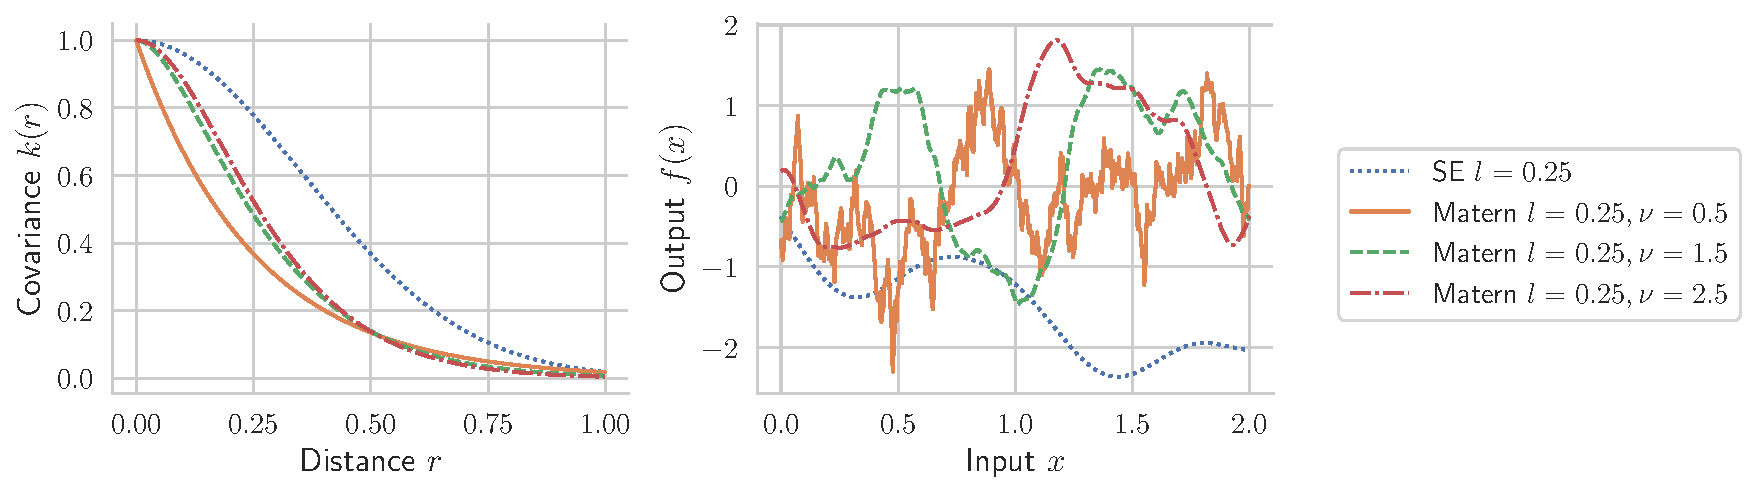
\includegraphics[width=\textwidth]{res/covariance_overview.pdf}
    \caption{Overview of different kernel functions. SE is squared exponential, $l$ is lengthscale, $\nu$ is the smoothness parameter. \textbf{Left}: covariance functions as function of distance. \textbf{Right}: prior functions $f \sim \mathcal N(\vect 0, K_{XX})$.}
    \label{fig:kernel_overview}
\end{figure}

\begin{figure}
    \centering
    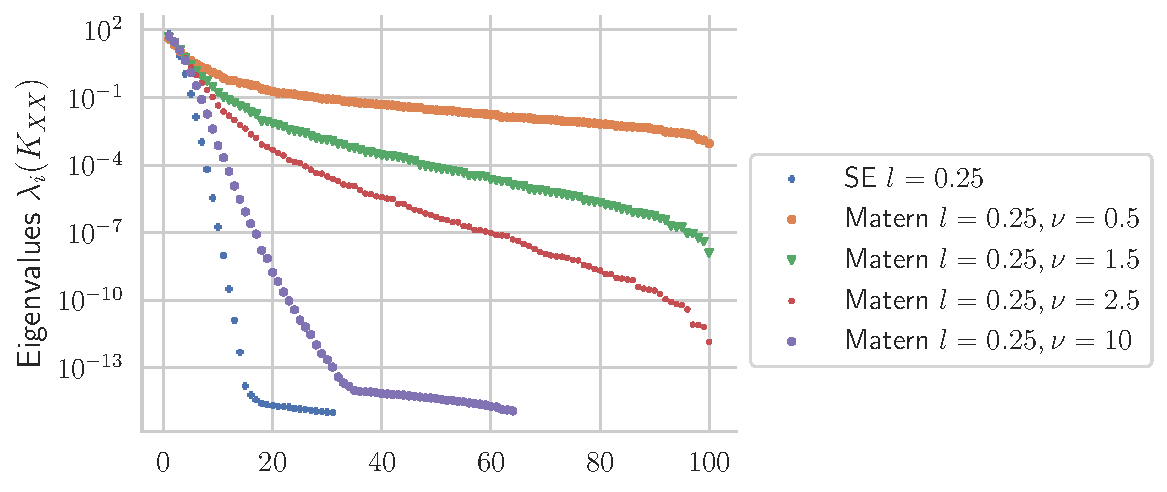
\includegraphics[width=0.6\textwidth]{res/kernel_eigenvalues.pdf}
    \caption{Eigenvalues of the kernel matrix $K_{XX}$ on a random grid $x_1, \ldots, x_{100} \sim \mathcal U([0, 1])$. Noise variance was set to $\sigma^2 = 0.1$.
    %Eigenvalues of the kernel matrix $K_{XX}$ on a uniform grid $x_i \in [0, 1], \, i = 1, \ldots, 100$. Eigenvalues below $10^{-15}$ were set to exactly zero.
    }
    \label{fig:kernel_mx_eigvals}
\end{figure}

\begin{figure}
    \centering
    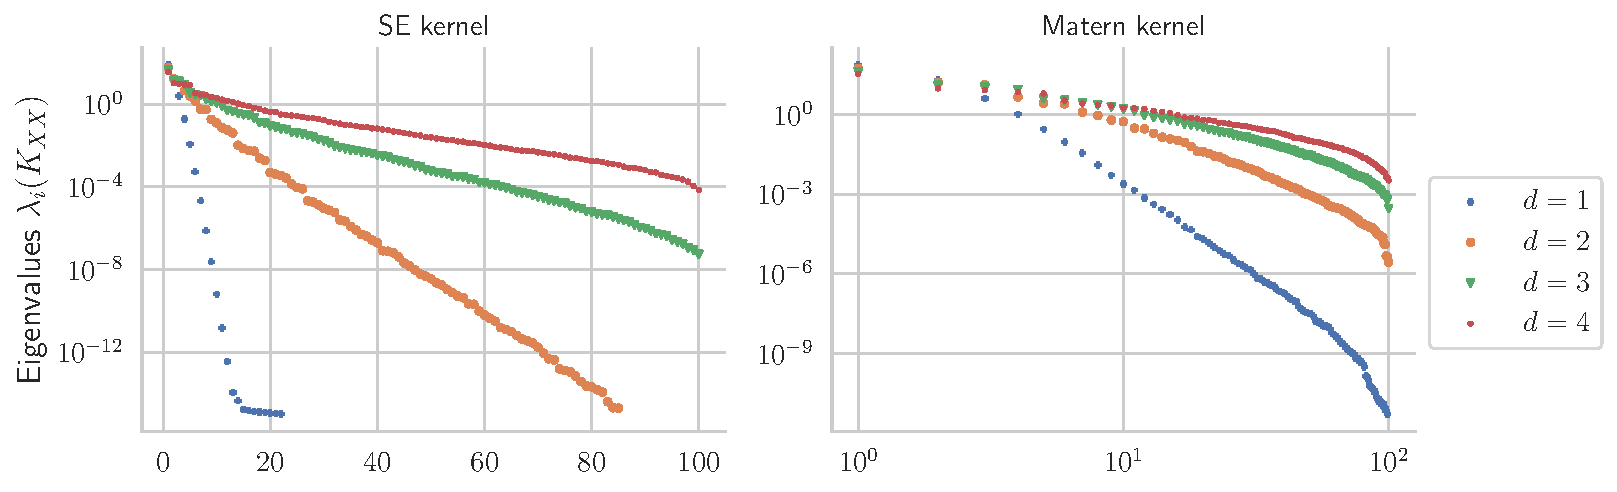
\includegraphics[width=0.85\textwidth]{res/kernel_eigenvalues_dimension.pdf}
    \caption{Effect of the input space dimension on the spectral decay of the kernel matrix. The grids are $\vect x_1, \ldots, \vect x_{100} \sim \mathcal U([0, 1]^d)$, noise variance $\sigma^2 = 0.1$. \textbf{Left}: squared exponential kernel with lengthscale $l=0.5$. \textbf{Right}: Matern kernel with $l=0.5, \nu = 2.5$.}
    \label{fig:my_label}
\end{figure}

\subsection{Preconditioning Kernel Matrices}

We seek for empirical evidence of formula \eqref{eq:pivchol_trace_error} for SE and Matern kernels with nodes in $[0, 1]$ on the left panel of Figure~\ref{fig:kernel_precond}. Indeed, the error $\trace(E_k) = \trace(K_{XX} - L_k L_k^\top)$ --- which is available exactly from pivoted Cholesky algorithm --- decays exponentially fast with respect to the rank $k$. However, the rate of decay is dramatically affected by the kernel parameters: rough kernels (i.e., small $l$ and small $\nu$) converge more slowly. In turn, this exponential error decay leads to a condition number that converges exponentially fast to one (see Corollary \ref{thm:pivchol_precond}), as shown in the right panel of Figure~\ref{fig:kernel_precond}. As expected, preconditioning with pivoted Cholesky is extremely effective as long as $\trace(E_k)$ decays exponentially. 

We start by showing empirical evidence of formula , i.e. the exponential convergence of pivoted Cholesky algorithm as a low-rank approximation of SE and Matern kernel matrices. As shown in left panel of Figure~\ref{fig:kernel_precond}, the error $E_k = K_{XX} - L_kL_k^\top$ in terms the trace is a linear curve on a semi-log scale, so that $\trace(E_k) = \mathcal O(\alpha^{-k})$ for some $\alpha > 1$.

We start by showing the exponential decay of the error of the pivoted Cholesky algorithm with respect to the number of steps $k$ in the left panel of Figure~\ref{fig:kernel_precond}. As suggested by formula \ref{}

In Figure~\ref{fig:logdet_precond}, logdet relative error with respect to the number of probe vectors $N$ while comparing different ranks of the preconditionner. For a fixed rank $k$ of the preconditionner, the relative error decreases with a rate about $\mathcal O(N^{-1/2})$. However, it is clear that the rank $k$ plays a much more important role for the error. Recall that the log-det is the sum of two values,

\begin{equation*}
    \log \det \widehat K_{XX} = \log\det\left(\widehat P_k^{-1} \widehat K_{XX} \right) + \log\det \widehat P_k \; ,
\end{equation*}

where randomness only occurs in the log-det of the preconditionned matrix, whereas $\log\det \widehat P_k$ is computed exactly. Since the preconditionned matrix converges quickly to the identity for even small values of $k$, its logdet will have small fluctuations around zero, so that the randomness incurred by the number of probe vectors has a small effect on the relative error.

\begin{comment}

\begin{figure}
    \centering
    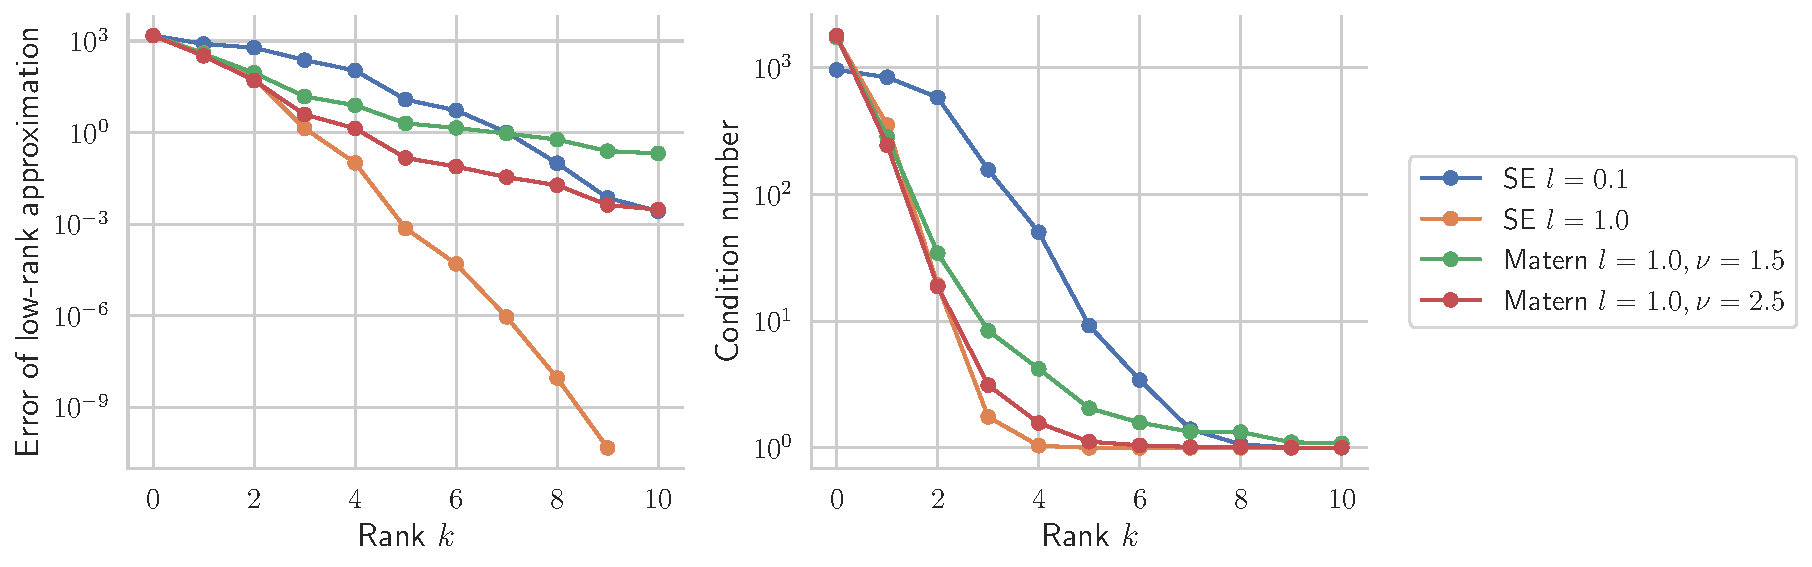
\includegraphics[width=\linewidth]{res/kernel_preconditionning.pdf}
    \caption{Preconditioning of kernel matrices with partial pivoted Cholesky. The preconditionner is $\widehat P_k = L_k L_k^\top + \sigma^2 \mathbb I$, 
    % NOTE: for some reason, my \Id command produces an error in the figure environment :( using hard-coded mathbb instead
    where $L_kL_k^\top \approx K_{XX}$. Kernels are univariate with data points $x_1, \ldots, x_{1000} \sim \mathcal U([0,1])$, the noise variance was set to $\sigma^2 = 0.5$. $k = 0$ denotes absence of preconditionning.
    \textbf{Left}: trace of error term $K_{XX} - L_k L_k^\top$. \textbf{Right}: condition number of the preconditionned SPD matrix $\widehat P_k^{-1/2} \widehat K_{XX} \widehat P_k^{-1/2}$.}
    \label{fig:kernel_precond}
\end{figure}

\end{comment}


\begin{figure}[ht!]
    \centering
    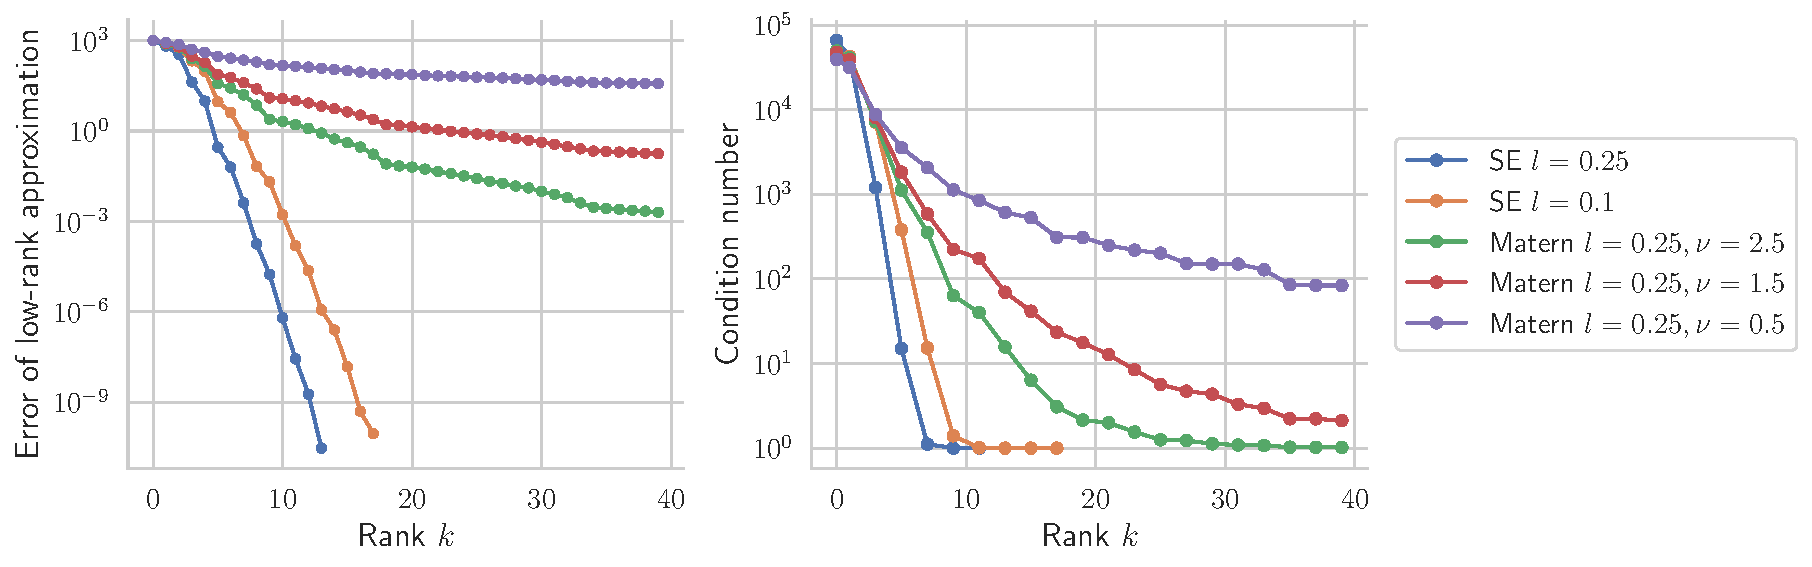
\includegraphics[width=0.9\linewidth]{report/res/kernel_preconditionning_1d_uniform.pdf}
    \caption{Preconditioning of kernel matrices with partial pivoted Cholesky. The preconditionner is $\widehat P_k = L_k L_k^\top + \sigma^2 \mathbb I$, 
    % NOTE: for some reason, my \Id command produces an error in the figure environment :( using hard-coded mathbb instead
    where $L_kL_k^\top \approx K_{XX}$. Kernels are univariate on a uniform grid on $[0, 1]$ with $n = 1000$ points, the noise variance was set to $\sigma^2 = 0.5$. $k = 0$ denotes absence of preconditionning.
    \textbf{Left}: trace of error term $K_{XX} - L_k L_k^\top$. \textbf{Right}: condition number of the preconditionned SPD matrix $\widehat P_k^{-1/2} \widehat K_{XX} \widehat P_k^{-1/2}$.}
    \label{fig:kernel_precond_1d_unif}
\end{figure}

\begin{figure}[h!]
    \centering
    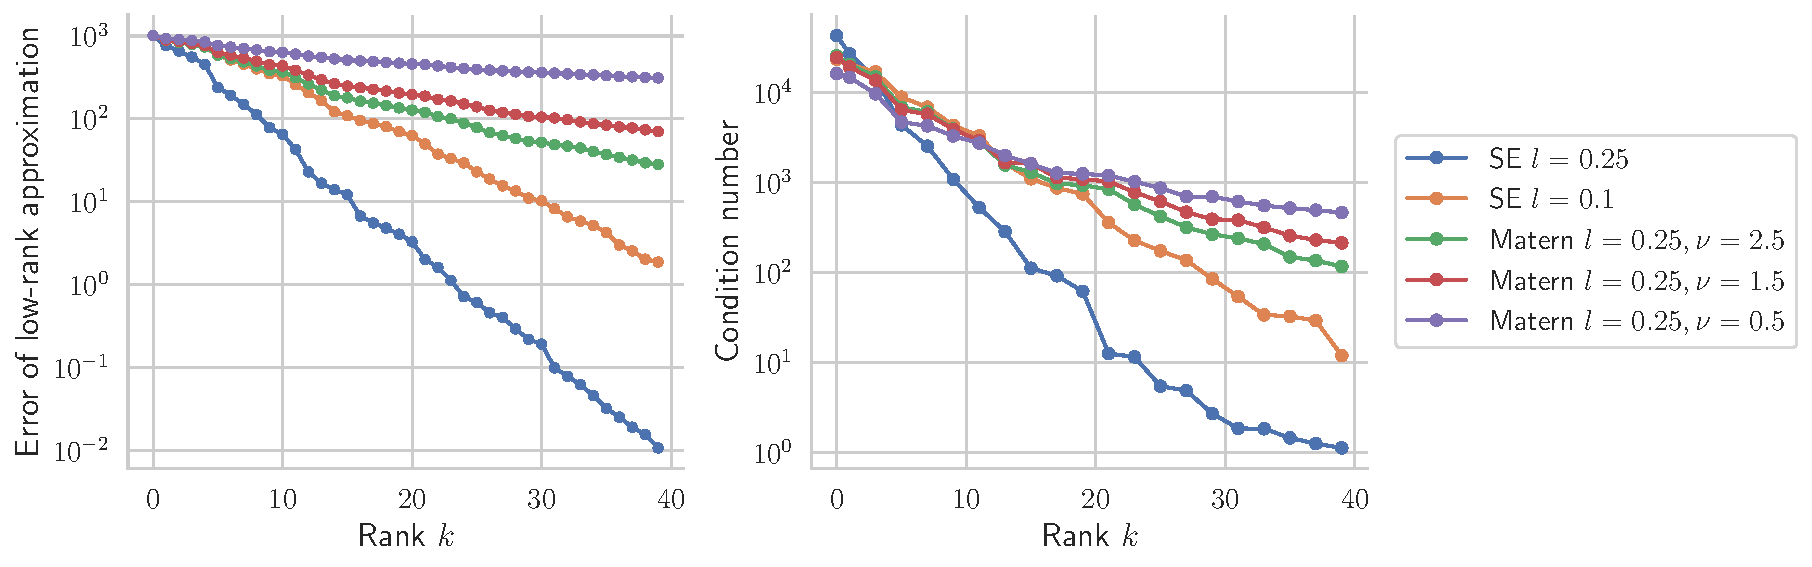
\includegraphics[width=0.9\linewidth]{report/res/kernel_preconditionning_2d_uniform.pdf}
    \caption{Same as Figure~\ref{fig:kernel_precond_1d_unif} but with 2-dimensional data $\vect x_1, \ldots, \vect x_{100} \sim \mathcal U([0, 1]^2)$.}
    \label{fig:kernel_precond_2d_unif}
\end{figure}


\begin{figure}[h!]
    \centering
    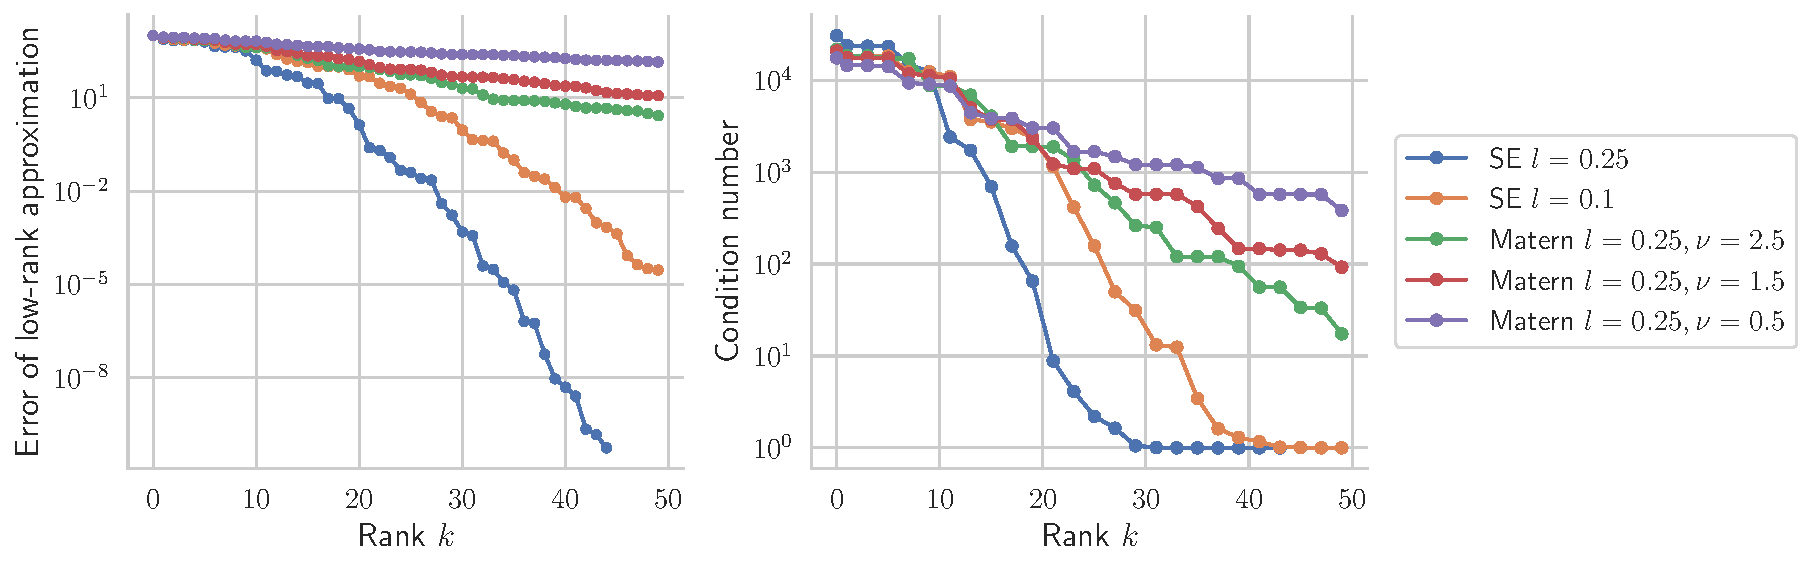
\includegraphics[width=0.9\linewidth]{report/res/kernel_preconditionning_1d_stdnormal.pdf}
    \caption{Same as Figure~\ref{fig:kernel_precond_1d_unif} but with 1-dimensional normally distributed data $\vect x_1, \ldots, \vect x_{100} \sim \mathcal N(0, 1)$.}
    \label{fig:kernel_precond_1d_stdnormal}
\end{figure}


\begin{figure}[h!]
    \centering
    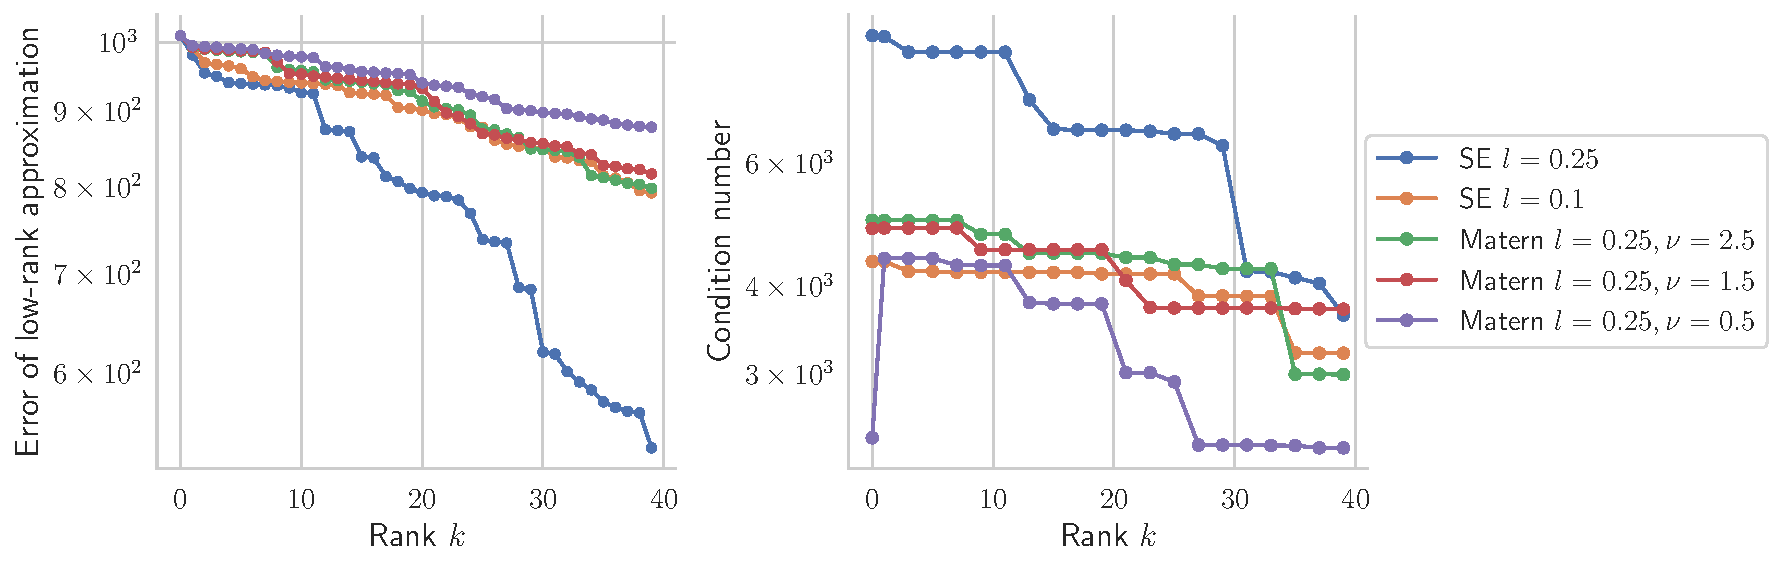
\includegraphics[width=0.9\linewidth]{report/res/kernel_preconditionning_2d_stdnormal.pdf}
    \caption{Same as Figure~\ref{fig:kernel_precond_1d_unif} but with 2-dimensional normally distributed data $\vect x_1, \ldots, \vect x_{100} \sim \mathcal N(\vect 0_2, \mathbb I_2)$.}
    \label{fig:kernel_precond_2d_stdnormal}
\end{figure}



\subsection{Stochastic Lanczos Quadrature for Log Determinant Estimation}

We start by log-det estimation without preconditioning. We show two cases in order to show the differences and how the number of Lanczos steps $m$ interplays with the number of probe vectors $N$ and the relative error $\epsilon$. Recall for a fixed error $\epsilon$, the estimated $N$ from Theorem \ref{thm:cortinovis} is mainly driven by $\norm{\log A}_F^2 / \trace(\log A)^2$. Hence, a matrix whose logdet is easy to compute should have its trace large compared to the variance of its trace estimator. The above ratio is minimized when the matrix has a single distinct eigenvalue. However, Lanczos would converge after a single iteration, so we instead set $\lambda_i = i$ in order to compare accuracy with respect to different number of steps. In the left panel of Figure~\ref{fig:logdet_mbcg}, we indeed see that the target error is reached with $m, N$ much smaller than their value estimated from Theorem \ref{thm:cortinovis}. Since the variance of the estimator is much smaller than the logdet, ...

In the left panel of Figure~\ref{fig:logdet_mbcg}, we see that 

\begin{figure}
    \centering
    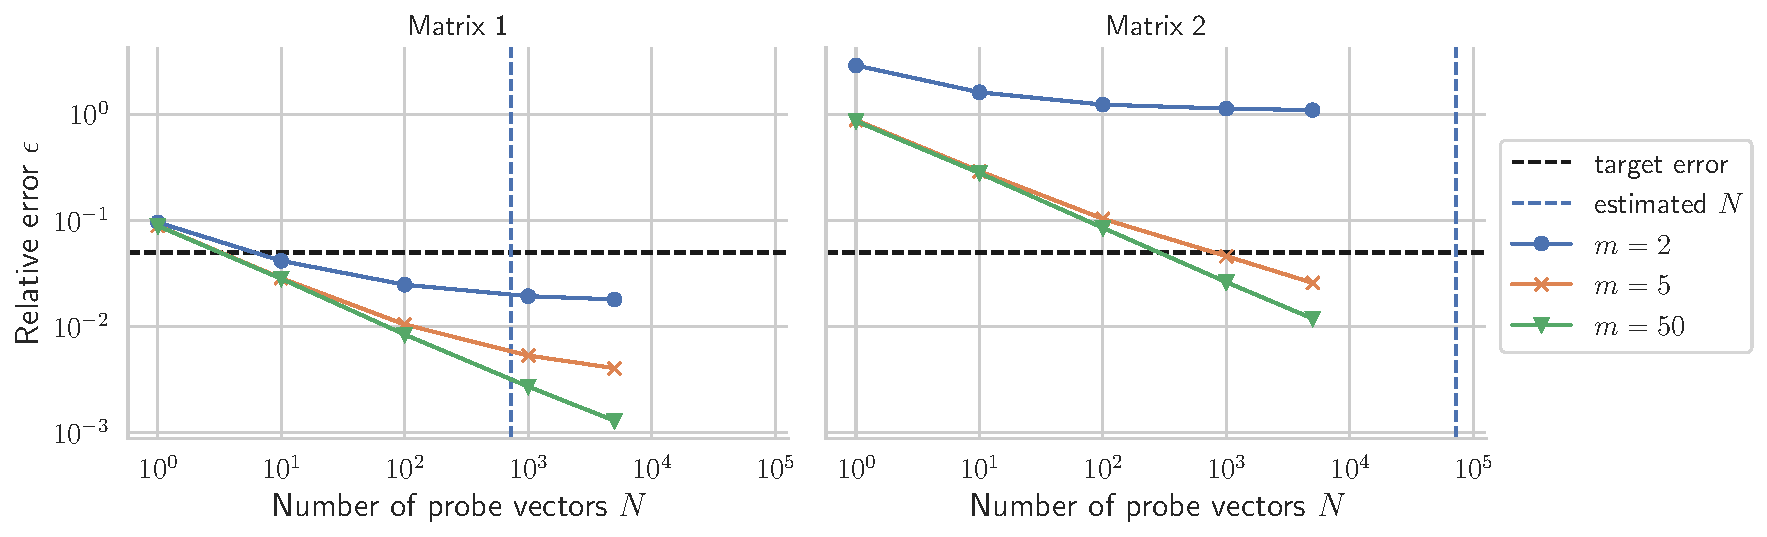
\includegraphics[width=\textwidth]{res/logdet_mbcg.pdf}
    \caption{Log determinant estimation with stochastic Lanczos quadrature where partial tridiagonal matrices were computed with mBCG algorithm. The matrices are $A = Q \Lambda Q^\top \in \R^{n \times n}$ with $n=1000$, $Q$ orthogonal and $\Lambda = \text{diag}(\lambda_1, \ldots, \lambda_n)$. The $95^\text{th}$ error quantiles are plotted. \textbf{Left}: $\lambda_i = i, \, 1 \le i \le n$, the estimated $m$ value is 51. \textbf{Right}: $\lambda_i = 10i, \, 1 \le i \le 10$, $\lambda_i = 1, \, 10 < i \le n$, so that $\text{rank}(\log K_{XX}) = 10$. The estimated $m$ value is $132$.}
    \label{fig:logdet_mbcg}
\end{figure}


\subsection{Logdet Estimation of Kernel Matrix with Preconditioning}

\begin{figure}
    \centering
    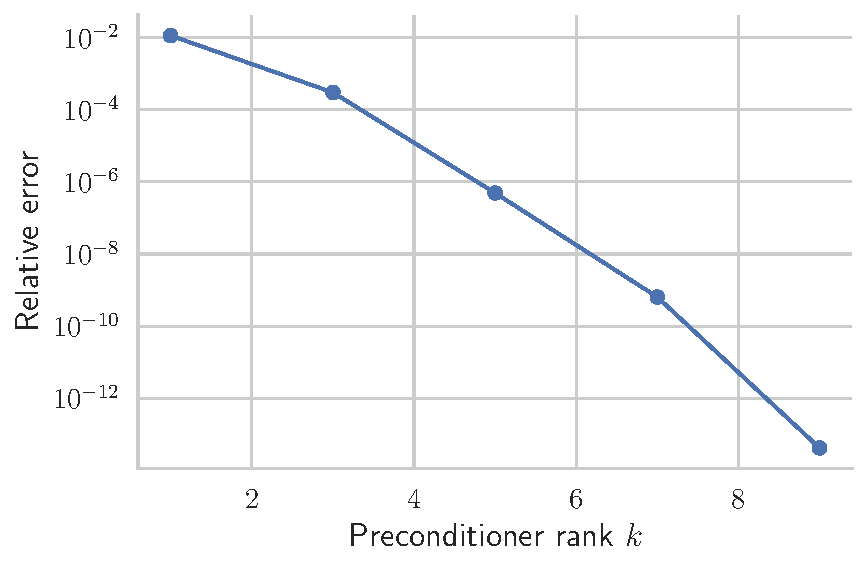
\includegraphics[width=0.5\textwidth]{res/logdet_precond_errvsk.pdf}
    \caption{Log determinant estimation of Kernel matrix with preconditioning. The kernel matrix is the SE kernel on the uniform grid $x_1, \ldots, x_n \in [0, 1], \, n=100$. The logdet is $\log\det \widehat K_{XX} = \log\det \widehat P_k + \log\det(\widehat P^{-1} \widehat K_{XX})$ where the logdet of the preconditioned matrix is computed with stochastic Lanczos quadrature. $N=100$ probe vectors are used and $m$ is large enough to reach tolerance $10^{-10}$.}
    \label{fig:my_label}
\end{figure}


\begin{figure}
    \centering
    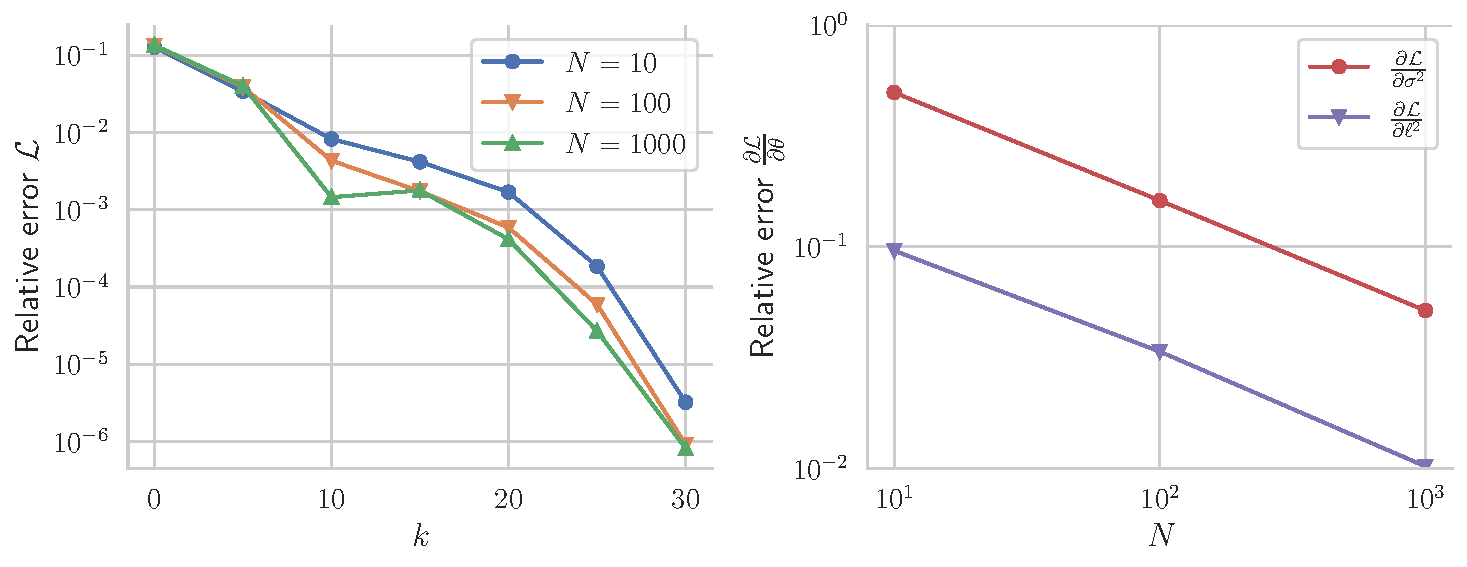
\includegraphics[width=0.9\textwidth]{report/res/likelihood.pdf}
    \caption{Average error and timing benchmark of the marginal log likelihood ($\mathcal L$) computed from mBCG output with pivoted Cholesky preconditioning over 10 runs. The data is $x_1, \ldots, x_{1000} \sim \mathcal U([0, 1]), \, y_i = \sin(2\pi x_i)$. mBCG steps $m$ was left unspecified to reach tolerance $10^{-10}$. Kernel parameters: $l = 0.25, \, \nu = 2.5$.}
    \label{fig:likelihood}
\end{figure}

\begin{figure}
    \centering
    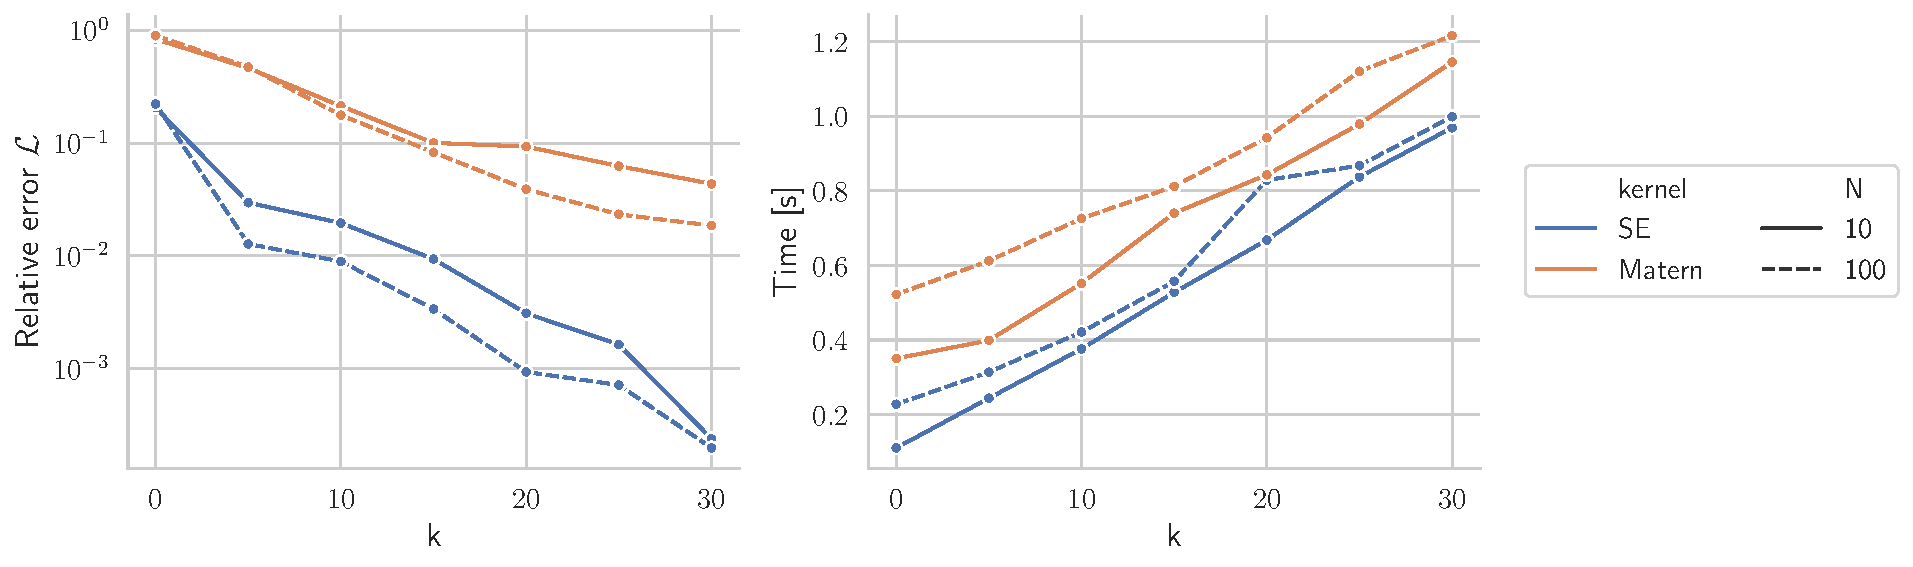
\includegraphics[width=0.9\textwidth]{report/res/likelihood_2d_unif.pdf}
    \caption{Same as Figure \ref{fig:likelihood} but with data $\sim \mathcal U([0,1]^2)$.}
    \label{fig:likelihood_2d_unif}
\end{figure}

\begin{figure}
    \centering
    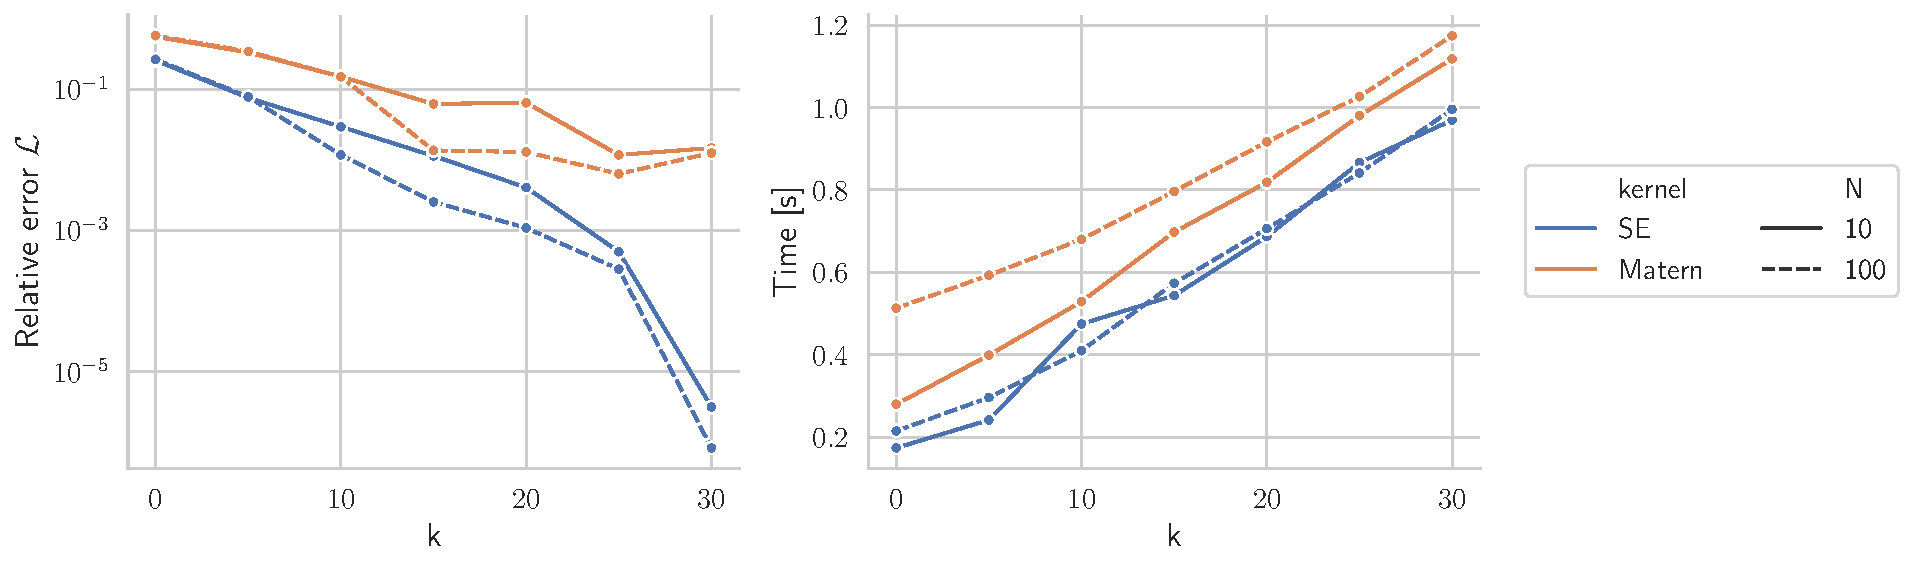
\includegraphics[width=0.9\textwidth]{report/res/likelihood_1d_stdnormal.pdf}
    \caption{Same as Figure \ref{fig:likelihood} but with data $\sim \mathcal N(0, 1)$.}
    \label{fig:likelihood_1d_stdnormal}
\end{figure}


%\subsection{"Logdet of precond captures everything when $k$ scales as log of ..."}

\begin{figure}
    \centering
    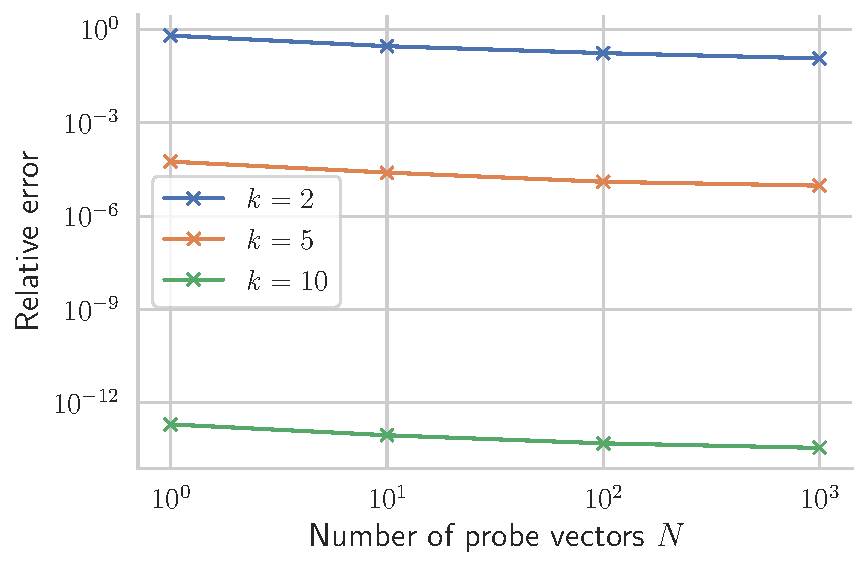
\includegraphics[width=0.5\textwidth]{res/logdet_precond.pdf}
    \caption{Caption}
    \label{fig:logdet_precond}
\end{figure}


% ----------------------------------------------


\newpage
\printbibliography


% ----------------------------------------------
\newpage
\appendix
\appendixpage

\section{Appendix - Gradient of Marginal Log-Likelihood} \label{sec:marginal_log_likelihood_gradient}

Starting from the marginal log-likelihood \eqref{eq:marginal_log_likelihood}, we wish to calculate the expression of its gradient with respect to hyperparameters $\theta_i$. We first compute the derivative of the inverse of a matrix using the chain rule,

\begin{equation*}
    \mymathbb 0 = \frac{d}{d \theta} \Id = \frac{d}{d \theta} \left( A^{-1}(\theta) A(\theta) \right) = \frac{d A^{-1}(\theta)}{d \theta} A(\theta) + A^{-1}(\theta) \frac{d A(\theta)}{d \theta}
     \;,
\end{equation*}

which yields

\begin{equation*}
    \frac{d A^{-1}(\theta) }{d \theta} = - A^{-1}(\theta) \frac{d A(\theta)}{d \theta} A^{-1}(\theta) \; .
\end{equation*}


The derivative of the determinant can be obtained with the Jacobi's formula %\textbf{TODO should I prove it? quite beautiful proof! recall NIDS lecture for polynomial invariants of deg > 3}
,

\begin{equation*}
    \frac{d}{d \theta} \det A(\theta) = \det (A(\theta)) \cdot \trace \left( A^{-1}(\theta) \frac{d A(\theta)}{d \theta} \right) \; .
\end{equation*}

Applying it on the log determinant will cancel the $\det A(\theta)$ term. We retrieve Equation \eqref{eq:marginal_log_likelihood_gradient} by substitution of the above quantities for $A(\theta) := \widehat K_{XX}$ where the dependence of the kernel on hyperparameters is left implicit for notation simplicity.


\section{Appendix --- Algorithms}

We first recall the Lanczos algorithm for linear systems and the preconditioned conjugate gradients algorithm. This introduces notation and serves as a reference for the derivation of Lanczos from CG as described in section \ref{sec:lanczos_from_cg}. We then present the mBCG algorithm, which combines Lanczos and CG extended to multiple right-hand sides, the reader can then spot differences with vanilla CG. We also provide a detailed explanation of batched computations for mBCG, both in terms of mathematical notation and programmatic implementation. 


\vspace{0.5cm}

\begin{algorithm}[H]
 \label{algo:lanczos}
\SetAlgoLined
\SetKwInOut{Input}{Input}
\SetKwInOut{Output}{Output}
\DontPrintSemicolon
\Input{matrix-vector multiplication oracles $\vect a \mapsto \widehat K_{XX} \vect a$, right-hand side $\vect b$, starting vector $\vect u_0$, number of steps $m$}
\Output{approximate solution $\vect u_m \approx \widehat K_{XX}^{-1} \vect b$, orthonormal basis $V_m$, tridigonal matrix $T_m$}
 %\tcp{Initialize residuals}
 $\vect r_0 \leftarrow \vect b - \widehat K_{XX} \vect x_0, \; \beta \leftarrow \norm{\vect r_0}_2$ \;
 %\tcp{Initialize basis for Krylov subspace}
 $\vect v_1 \leftarrow \vect r_0 / \beta$ \;
 \For{$k = 1, \ldots, m$}{
    $\tilde{\vect w} \leftarrow \widehat K_{XX} \vect v_k - \eta_k \vect v_{k-1}$ \tcp*{if k=1, set $\eta_1 \vect v_0 := \vect 0$}
    $\delta_k \leftarrow \vect v_k^\top \tilde{\vect w}$ \;
    $\vect w_k \leftarrow \tilde{\vect w} - \delta_k \vect v_k$ \;
    $\eta_k \leftarrow \norm{\vect w_k}_2$ \;
    $\vect v_{k+1} \leftarrow \vect w_l / \eta_k$ \; 
 }
 $V_m = \begin{bmatrix} \vect v_1 & \dots & \vect v_m \end{bmatrix}, \; T_m = \text{tridiag}(\eta_{k-1}, \delta_k, \eta_k)$ \;
 Compute $\vect y_m = \beta T_m^{-1} \vect e_1$ and $\vect u_m = \vect u_0 + V_m \vect y_m$ \;
 
 \caption{Lanczos algorithm to solve linear system $\widehat K_{XX} \vect u = \vect b$}
\end{algorithm}


\begin{algorithm}[H]
 \label{algo:pcg}
\SetAlgoLined
\SetKwInOut{Input}{Input}
\SetKwInOut{Output}{Output}
\DontPrintSemicolon
\Input{matrix-vector multiplication oracles $\vect a \mapsto \widehat K_{XX} \vect a$ and $\vect a \mapsto P^{-1} \vect a$, right-hand side $\vect b$, number of steps $m$}
\Output{approximate solution $\vect u_m \approx \widehat K_{XX}^{-1} \vect b$}
 \tcp{Initialize solution and residuals}
 $\vect u_0 \leftarrow \vect 0, \; \vect r_0 \leftarrow \vect b$ \;
 \tcp{Initialize preconditioned residuals and first search direction}
 $\vect z_0 \leftarrow P^{-1} \vect r_0$ \;
 $\vect d_1 \leftarrow \vect r_0$ \;
 
 \For{$k = 1, \ldots, m$}{
    \tcp{Line search: optimal step size in direction $\vect d_k$}
    $\alpha_k \leftarrow \vect r_k^\top \vect z_k \,/\, \vect d_k^\top (\widehat K_{XX} \vect d_k)$ \;
    \tcp{Update solution and residuals}
    $\vect u_k \leftarrow \vect u_{k-1} + \alpha_k \vect d_k$ \;
    $\vect r_k \leftarrow \vect r_{k-1} - \alpha_k \widehat K_{XX} \vect d_k$ \;
    $\vect z_k \leftarrow P^{-1} \vect r_k$ \;
    \tcp{Conjugate Gram Schmidt and compute next search direction}
    $\beta_k \leftarrow \vect r_k^\top \vect z_k \,/\, \vect r_{k-1}^\top \vect z_{k-1}$ \;
    $\vect d_{k+1} \leftarrow \vect z_k + \beta_k \vect d_k$ \;
 }
 \caption{Vanilla conjugate gradients to solve $\widehat K_{XX} \vect u = \vect b$}
\end{algorithm}

\vspace{0.5cm}

\begin{algorithm}[H]
 \label{algo:mBCG}
\SetAlgoLined
\SetKwInOut{Input}{Input}
\SetKwInOut{Output}{Output}
\DontPrintSemicolon
\Input{matrix-matrix multiplication oracles $A \mapsto \widehat K_{XX} A$ and $A \mapsto P^{-1} A$, right-hand side $B = \begin{bmatrix}
\vect y & \vect z_1 & \ldots & \vect z_N
\end{bmatrix}$, number of steps $m$}
\Output{approximate solutions $U_m \approx \widehat K_{XX}^{-1} B$, partial Lanczos tridiagonalizations $T_m^{(i)}$}
 \tcp{Initialize solutions and residuals}
 $U_0 \leftarrow \mymathbb 0_{n \times (N+1)}$ \;
 $R_0 \leftarrow B$ \;
 \tcp{Initialize preconditioned residuals and search directions}
 $Z_0 \leftarrow P^{-1} R_0$ \;
 $D_1 \leftarrow R_0$ \;
 \tcp{Initialize tridigonal matrices}
 $T_m^{(1)}, \ldots, T_m^{(N)} \leftarrow \mymathbb 0_{m \times m}$ \;
 \For{$k = 1, \ldots, m$}{
    \tcp{Line search: optimal step sizes in directions $D_k$}
    $\vect \alpha_k \leftarrow \varphi(R_k, Z_k) \, ./ \, \varphi(D_k, \widehat K_{XX} D_k)$ \;
    \tcp{Update solutions and residuals}
    $U_k \leftarrow U_{k-1} + D_k \, \text{diag}(\vect\alpha_k)$ \; % (\vect 1 \vect\alpha_k^\top) \odot D_k
    $R_k \leftarrow R_{k-1} - \widehat K_{XX} D_k \, \text{diag}(\vect \alpha_k)$ \; % (\vect 1 \vect\alpha_k^\top) \odot (\widehat K_{XX} D_k)
    $Z_k \leftarrow P^{-1} R_k$ \;
    \tcp{Conjugate Gram Schmidt and compute next search directions}
    $\vect\beta_k \leftarrow \varphi(R_k, Z_k) \,./\, \varphi(R_{k-1}, Z_{k-1})$ \;
    $D_{k+1} \leftarrow Z_{k} + D_k \, \text{diag}(\vect\beta_k)$ \; % (\vect 1 \vect\beta_k^\top) \odot D_k
    \tcp{Compute tridiagonal matrices}
    $[T_m^{(i)}]_{kk} \leftarrow 1 / [\vect \alpha_k]_i + [\vect\beta_{k-1}]_i / [\vect\alpha_{k-1}]_i, \quad i=1, \ldots, N$ \;
    $[T_m^{(i)}]_{k-1, k}, \, [T_m^{(i)}]_{k, k-1} \leftarrow \sqrt{[\vect\beta_{k-1}]_i} / [\vect\alpha_k]_i, \quad i=1, \ldots, N$ \;
 }
 \caption{mBCG to solve Equation \eqref{eq:mbcg_equation}}
\end{algorithm}

\vspace{0.5cm}

We discuss how $p$ right-hand sides can be handled simultaneously. Matrix-vector multiplication $\vect a_i \mapsto \widehat K_{XX} \vect a_i$ is trivially extended to matrix-matrix multiplication $A \mapsto \widehat K_{XX} A$ since

\begin{equation*}
    \widehat K_{XX} A = \widehat K_{XX} \begin{bmatrix}
    \vect a_1 & \dots & \vect a_p
    \end{bmatrix}  = \begin{bmatrix}
    \widehat K_{XX} \vect a_1 & \dots & \widehat K_{XX} \vect a_p
    \end{bmatrix} \; .
\end{equation*}

Vectors $\vect \alpha_k, \vect \beta_k \in \R^{p}$ store the coefficients at each step $k$ for the $p$ right-hand sides. Their computation involves the function $\varphi$ which simply generalizes dot products:

\begin{equation*}
    \varphi: \R^{n \times p} \times \R^{n \times p} \to \R^{p}, \quad
    \varphi(\begin{bmatrix}
    \vect a_1 & \dots & \vect a_p
    \end{bmatrix}, \begin{bmatrix}
    \vect b_1 & \dots & \vect b_p
    \end{bmatrix})
    = \begin{bmatrix}
    \vect a_1^\top \vect b_1 & \dots & \vect a_p^\top \vect b_p
    \end{bmatrix}^\top \; ,
\end{equation*}

which is programatically implemented as element-wise multiplication of $A$ and $B$ and then summing across the first dimension. The $./$ symbol then refers to element-wise division. Finally, note that 

\begin{equation*}
    A \, \text{diag}(\vect\alpha) = \begin{bmatrix} \alpha_1 \vect a_1 & \dots & \alpha_p \vect a_p \end{bmatrix}
\end{equation*}

simply weights columns of $A$ by coefficients in $\vect\alpha$. Explicit computation of the diagonal matrix is straightforward to avoid using Numpy's broadcasting rules\footnote{See \url{https://numpy.org/doc/stable/user/basics.broadcasting.html}}, e.g. \texttt{alpha.T * A}. 

\begin{comment}
Finally, denoting $\odot$ the element-wise multiplication and $\vect 1$ a vector full of ones, the expression

\begin{equation*}
    (\vect 1 \vect \alpha^\top) \odot A 
    = \begin{bmatrix}
    \alpha_1 \vect 1 & \dots & \alpha_p \vect 1
    \end{bmatrix} \odot \begin{bmatrix} \vect a_1 & \dots & \vect a_p \end{bmatrix}
    = \begin{bmatrix} \alpha_1 \vect a_1 & \dots & \alpha_p \vect a_p \end{bmatrix} \; ,
\end{equation*}

results in weighting each column of $A$ by coefficients in $\vect\alpha$. This is straightforward to implement using Numpy's broadcasting rules\footnote{See \url{https://numpy.org/doc/stable/user/basics.broadcasting.html}}, e.g. \texttt{alpha.T * A}. 
\end{comment}


\section{Questions}


\section{TODOs}

\subsection{Report}

\begin{itemize}
    \item Abstract
    \item \st{Introduction: Gaussian Process regression}. Keywords: non parametric, weight-space vs function space view, bayesian linear regression, kernel trick, notation for kernel matrix, feature space, distribution over functions, etc
    \begin{itemize}
        \item rewrite introduction of introduction
        \item probably too verbose...
    \end{itemize}
    \item Rewrite preconditionning section
    \item Numerical experiments
\end{itemize}

\subsection{Theory}

\begin{itemize}
    \item Lemma 4 of Gardner only for even polynomials ??? The  can only bound one out of two eigenvalues of the kernel matrix, what are the implications ?
    \item Try to apply lemmas to Matern kernels
    \item Try to apply lemmas to multivariate kernels
    \item Restate results for nodes in general interval $[a, b]$
    \item Thoughts for Matern kernels: we know the Fourier transform of the RBF and Matern kernels \cite{rasmussen_gaussian_2005}, using that the eigenvalues of the kernel matrix converges to the eigenvalues of the corresponding operator (e.g. \cite{braun_accurate_2006}), can we recover the eigenvalue decay from the Fourier transform ?
\end{itemize}

\subsection{Numerical experiments}

\begin{itemize}
    \item \st{Check bug in mBCG: bad convergence with log-uniform eigenvalues} 
    \begin{itemize}
        \item I have the same results as scipy's cg algorithm
        \item $\Rightarrow$ check literature
    \end{itemize}
    \item \st{Preconditionning of kernel matrices.} Done, Figure \ref{fig:kernel_precond}
    \item Convergence of logdet w.r.t. $N$, $m$, with preconditionning $\rightarrow$ also w.r.t. rank $k$
\end{itemize}

\textcolor{red}{DAVID'S LIST OF TO DO'S}
\begin{itemize}
    \item Introduction: Introduce GP inference and explain the problem, related work etc.
    \item Problem: Clearly state what you are trying to solve and how you arrive at this problem (derivation of MLE etc), and what you have achieved.
    \item Section of Monte carlo trace estimation. Include monte carlo bounds.
    \item Section on stochastic Lanczos. Include bounds that take into account lanczos. Explain problem when condition number is large and why we need preconditioning.
    \item Explain preconditioning. Include result on the condition number of RBF and Matern kernels. Restate theorem on how many matvecs you need to do to get a sufficiently accurate estimate. Explain sampling etc. 
    \item Final algorithm
    \item Numerical experiments.
    \item Conclusion
\end{itemize}

\end{document}
